Recovery and downblending of \gls{HEU} to produce \gls{HALEU} means that 
the fuel contains impurities present in the original
\gls{HEU}. Known impurities in potential \gls{HEU}
supplies to create \gls{HALEU} include $^{232}$U and $^{236}$U
\cite{vaden_isotopic_2018,nelson_foreign_2010},  
which are parasitic neutron absorbers and have the potential to affect 
reactor physics and reactor operation. To investigate the magnitude of this 
effect, this chapter presents models of two advanced reactors that use  
impure \gls{HALEU} fuel (with compositions based on publicly 
available information) and compares the performance of the impure 
fuel to the use of pure 
\gls{HALEU} (comprised exclusively of $^{235}$U and $^{238}$U). This analysis 
helps in understanding the impacts of the impurities on the performance 
of the reactor. While the other chapters of this dissertation explore 
how the reactors affect the fuel cycle this chapter explores how the 
fuel affects the reactors.  

\section{Methodology}\label{sec:neutronics-methods}
For this work we considered the two \gls{HALEU}-fueled reactors modeled 
in the transition scenarios described in Chapter \ref{ch:fc_methods}: the 
X-energy Xe-100 and the \gls{USNC} \gls{MMR}. We created reactor 
core models that closely resemble these reactors in Serpent 
\cite{leppanen_serpent_2014}, modeling the neutronics and fuel depletion  
in each reactor design. Each model was run using the ENDF VII.1 
cross section library
\cite{chadwick_endfb-vii1_2011}. The core geometries used are not 
the exact geometries designed by X-energy and \gls{USNC}, respectively, but 
are replications based on publicly-available information 
\cite{mulder_overview_2021,nuscale_chapter_2020,reyes_nuscale_2021,reyes_correction_2022}. 
We used the serpentTools python package \cite{johnson_serpenttools_2020} to 
analyze the results from the models.

\subsection{Xe-100-like model} \label{sec:xe100_serpent_model}
The Xe-100 is a 200 MWth, 80 MWe, \acrfull{TRISO}-fueled pebble-bed 
\gls{HTGR} \cite{mulder_overview_2021}. To model this reactor
we used the Sanagmon200 model from \cite{richter_isotopic_2022}, shown in 
Figure \ref{fig:xe100_core}, to serve as an Xe-100-like 
core model. The model itself can be found on GitHub \cite{richter_zoerichterphlox_2022}.
The Sangamon200 model is a \acrfull{TRISO}-fueled, pebble-bed, \gls{HTGR}-style 
reactor core model initially created to characterize the isotopic 
compositions and reactor physics of a 200 MWth pebble-bed \gls{HTGR}. 

\begin{figure}[ht]
    \centering 
    \begin{subfigure}{0.45\textwidth}
        \centering 
        \includegraphics[scale=0.03]{htgr-mr-full-core.inp_geom1.png}
        \caption{Radial view of Xe-100-like core model.}
        \label{fig:xe100_core_radial}        
    \end{subfigure}
    \hfill
    \begin{subfigure}{0.45\textwidth}
        \centering 
        
\includegraphics[scale=0.12]{htgr-mr-full-core.inp_geom3.png}
        \caption{Axial view of Xe-100-like core model.}
        \label{fig:xe100_core_axial}        
    \end{subfigure}
    \caption{Xe-100-like core model made in Serpent.}
    \label{fig:xe100_core}
\end{figure}
While this reactor model 
is very similar to current published data for the X-energy Xe-100
\cite{mulder_overview_2021}, there are two notable differences that affect 
the reactor physics. The first difference is that the \gls{TRISO} particles 
in the Sangamon200 are modeled as a blended mix of the \gls{TRISO} 
materials and not the explicit layers. Using a homogenized \gls{TRISO} particle 
decreases the \keff of the core by 4.45\%, but it does not reduce the 
thermal and fast neutron fluxes across the reactor outside of error 
\cite{richter_isotopic_2022}. Despite 
the effect on \keff of this modeling decision, we used the 
homogenized model of the \gls{TRISO} pebbles to be consistent with the 
published results of the Sanagamon200 \cite{richter_isotopic_2022} and 
to be conscious of computational expense. 
The second 
notable difference is the reactor vessel shape. The Sanagmon200 is a simple 
cylinder, while the Xe-100 is a cylinder with a cone at the bottom to funnel 
the pebbles to a single point as they come out of the core. However, 
this is a less neutronically important region of the core, and we kept the 
geometry of the Sangamon200 for consistency with those published results. 

In the Xe-100 reactor, each pebble moves down the core while it burns. Each 
time that a pebbles travels from the top of the core to the bottom is a single 
pass. Once a pebble reaches the bottom of the core, it is removed, inspected for 
the burnup level, and placed back in the core for another pass if the pebble has 
not reached the target burnup. Each pebble is expected to 
go through multiple passes in the core, an average 
of six passes per pebble, before reaching the target burnup of 185 
MWd/kg. To account for the different burnup of 
the pebbles in an equilibrium core, 
six different pebble isotopic compositions were used to approximate the pebble
variance in burnup in the core. These isotopic compositions represent burnup from 
integer numbers of passes through the core.
To determine the isotopic composition of the 
pebbles after each pass we performed the methodology 
Richter developed for their modeling of the Sangamon200 \cite{richter_isotopic_2022}. 
We performed depletion on the single pebble model created by Richter 
\cite{richter_zoerichterphlox_2022},
with each layer of the \gls{TRISO} kernel explicitly modeled
with depletion steps 
corresponding to integer numbers of passes. Then we 
applied the composition corresponding to the burnup step of each pass 
to 1/6th of the pebbles of the core. The pebbles with different burnups 
were mixed throughout the core, mimicking the spread of 
differently burned pebbles throughout a core in the equilibrium state 
of the reactor. Each pebble at the same burnup level has the same 
composition in this model.   

The Sangamon200 in an an isothermal state at 800 K 
\cite{richter_isotopic_2022}.
We ran this model with 100,000 particles per cycle, 50 inactive cycles, 
and 200 active cycles without modeling depletion on the Sangamon200 model 
because our model does not capture pebble movement or the continuous 
refueling scheme used by the Xe-100. Performing depletion without modeling 
pebble movement 
would create non-physical differences from the equilibrium condition of 
this reactor model. Therefore, we did not model further depletion of the 
pebbles when comparing the different fuel compositions.

\subsection{MMR-like model}
The \gls{USNC} \gls{MMR} is a 15 MWth, 5 MWe, prismatic \gls{HTGR} that 
uses \gls{TRISO} fuel in \acrfull{FCM} pellets inside graphite blocks 
\cite{noauthor_usnc_2021}.
We created an \gls{MMR}-like model primarily based on information in 
\cite{hawari_development_2018}, and supplemented or modified based on 
information published by \gls{USNC} \cite{noauthor_usnc_2021}. 
Information about the \gls{TRISO} 
particle and \gls{FCM} pellets was found in \cite{noauthor_usnc_2021}
and information about the graphite block dimensions and configuration 
was found via visual inspection of figures in \cite{venneri_micro_2019}. 
The final core configuration 
is different than what is modeled by Hawari and Venneri \cite{hawari_development_2018} 
because their model is only meant to operate 
for 10 years, while the \gls{MMR} is meant to operate for 20 years 
\cite{noauthor_usnc_2021}. We selected the core configuration shown in 
Figure \ref{fig:mmr_core} after modeling some of the other core 
configurations found in literature \cite{mitchell_usnc_2020,hawari_development_2018}
and determining that the selected core configuration  
can operate the longest before going subcritical and 
achieve a burnup close to the reported 82.6 MWd/kgU reported by 
\gls{USNC} \cite{noauthor_usnc_2021}. 

Figure \ref{fig:mmr_core} shows a radial and axial slice of the 
\gls{MMR} model. The fuel channels have a radius of 1.15 cm, the same
size as the \gls{FCM} pellets based on no other available information, 
the coolant channels have a radius of 
3 cm, arbitrarily chosen because no specific information was found, 
and the control rod channels have a radius of 6 cm, obtained from 
\cite{hawari_development_2018}. These dimensions affect the graphite volume 
of the core, and thus affect the fuel to moderator ratio of the core. 
The \gls{TRISO} particles are modeled with a 40\% packing fraction in 
the \gls{FCM} particles \cite{powers_fully_2014}.
Control rods and burnable poisons are not included in this model, or 
the Sangamon200 model, so the control rod locations are filled with helium.
There are five layers of the graphite fuel blocks 
stacked to form the entire core, to approximate the number of 
fuel blocks described in \cite{noauthor_usnc_2021}. The entire core 
is assumed to be in an isothermal state at 800 K. There is a 20 cm 
thick graphite reflector above and below the stacks of graphite, 
and a 10 cm thick beryllium-oxide reflector on the outside of the 
graphite blocks of the core, illustrated by the green material in 
Figure \ref{fig:mmr_core}. While Hawari and Venneri \cite{hawari_development_2018}
define both of these reflectors in their model, they only 
define the thickness of the beryllium-oxide reflector. Therefore we 
assumed a graphite reflector thickness of 20 cm to provide 3-5 mean 
free paths of material. The input files for this model can be found at 
\cite{bachmann_mmr-like_2023}.

\begin{figure}
        \begin{subfigure}{0.48\textwidth}
                \centering
                
\includegraphics[scale=0.15]{bachmann-mmr_geom1.png}
                \caption{Radial view of the USNC MMR-like model.}
                \label{fig:mmr_radial}
        \end{subfigure}
        \hfill 
        \begin{subfigure}{0.48\textwidth}
                \centering
                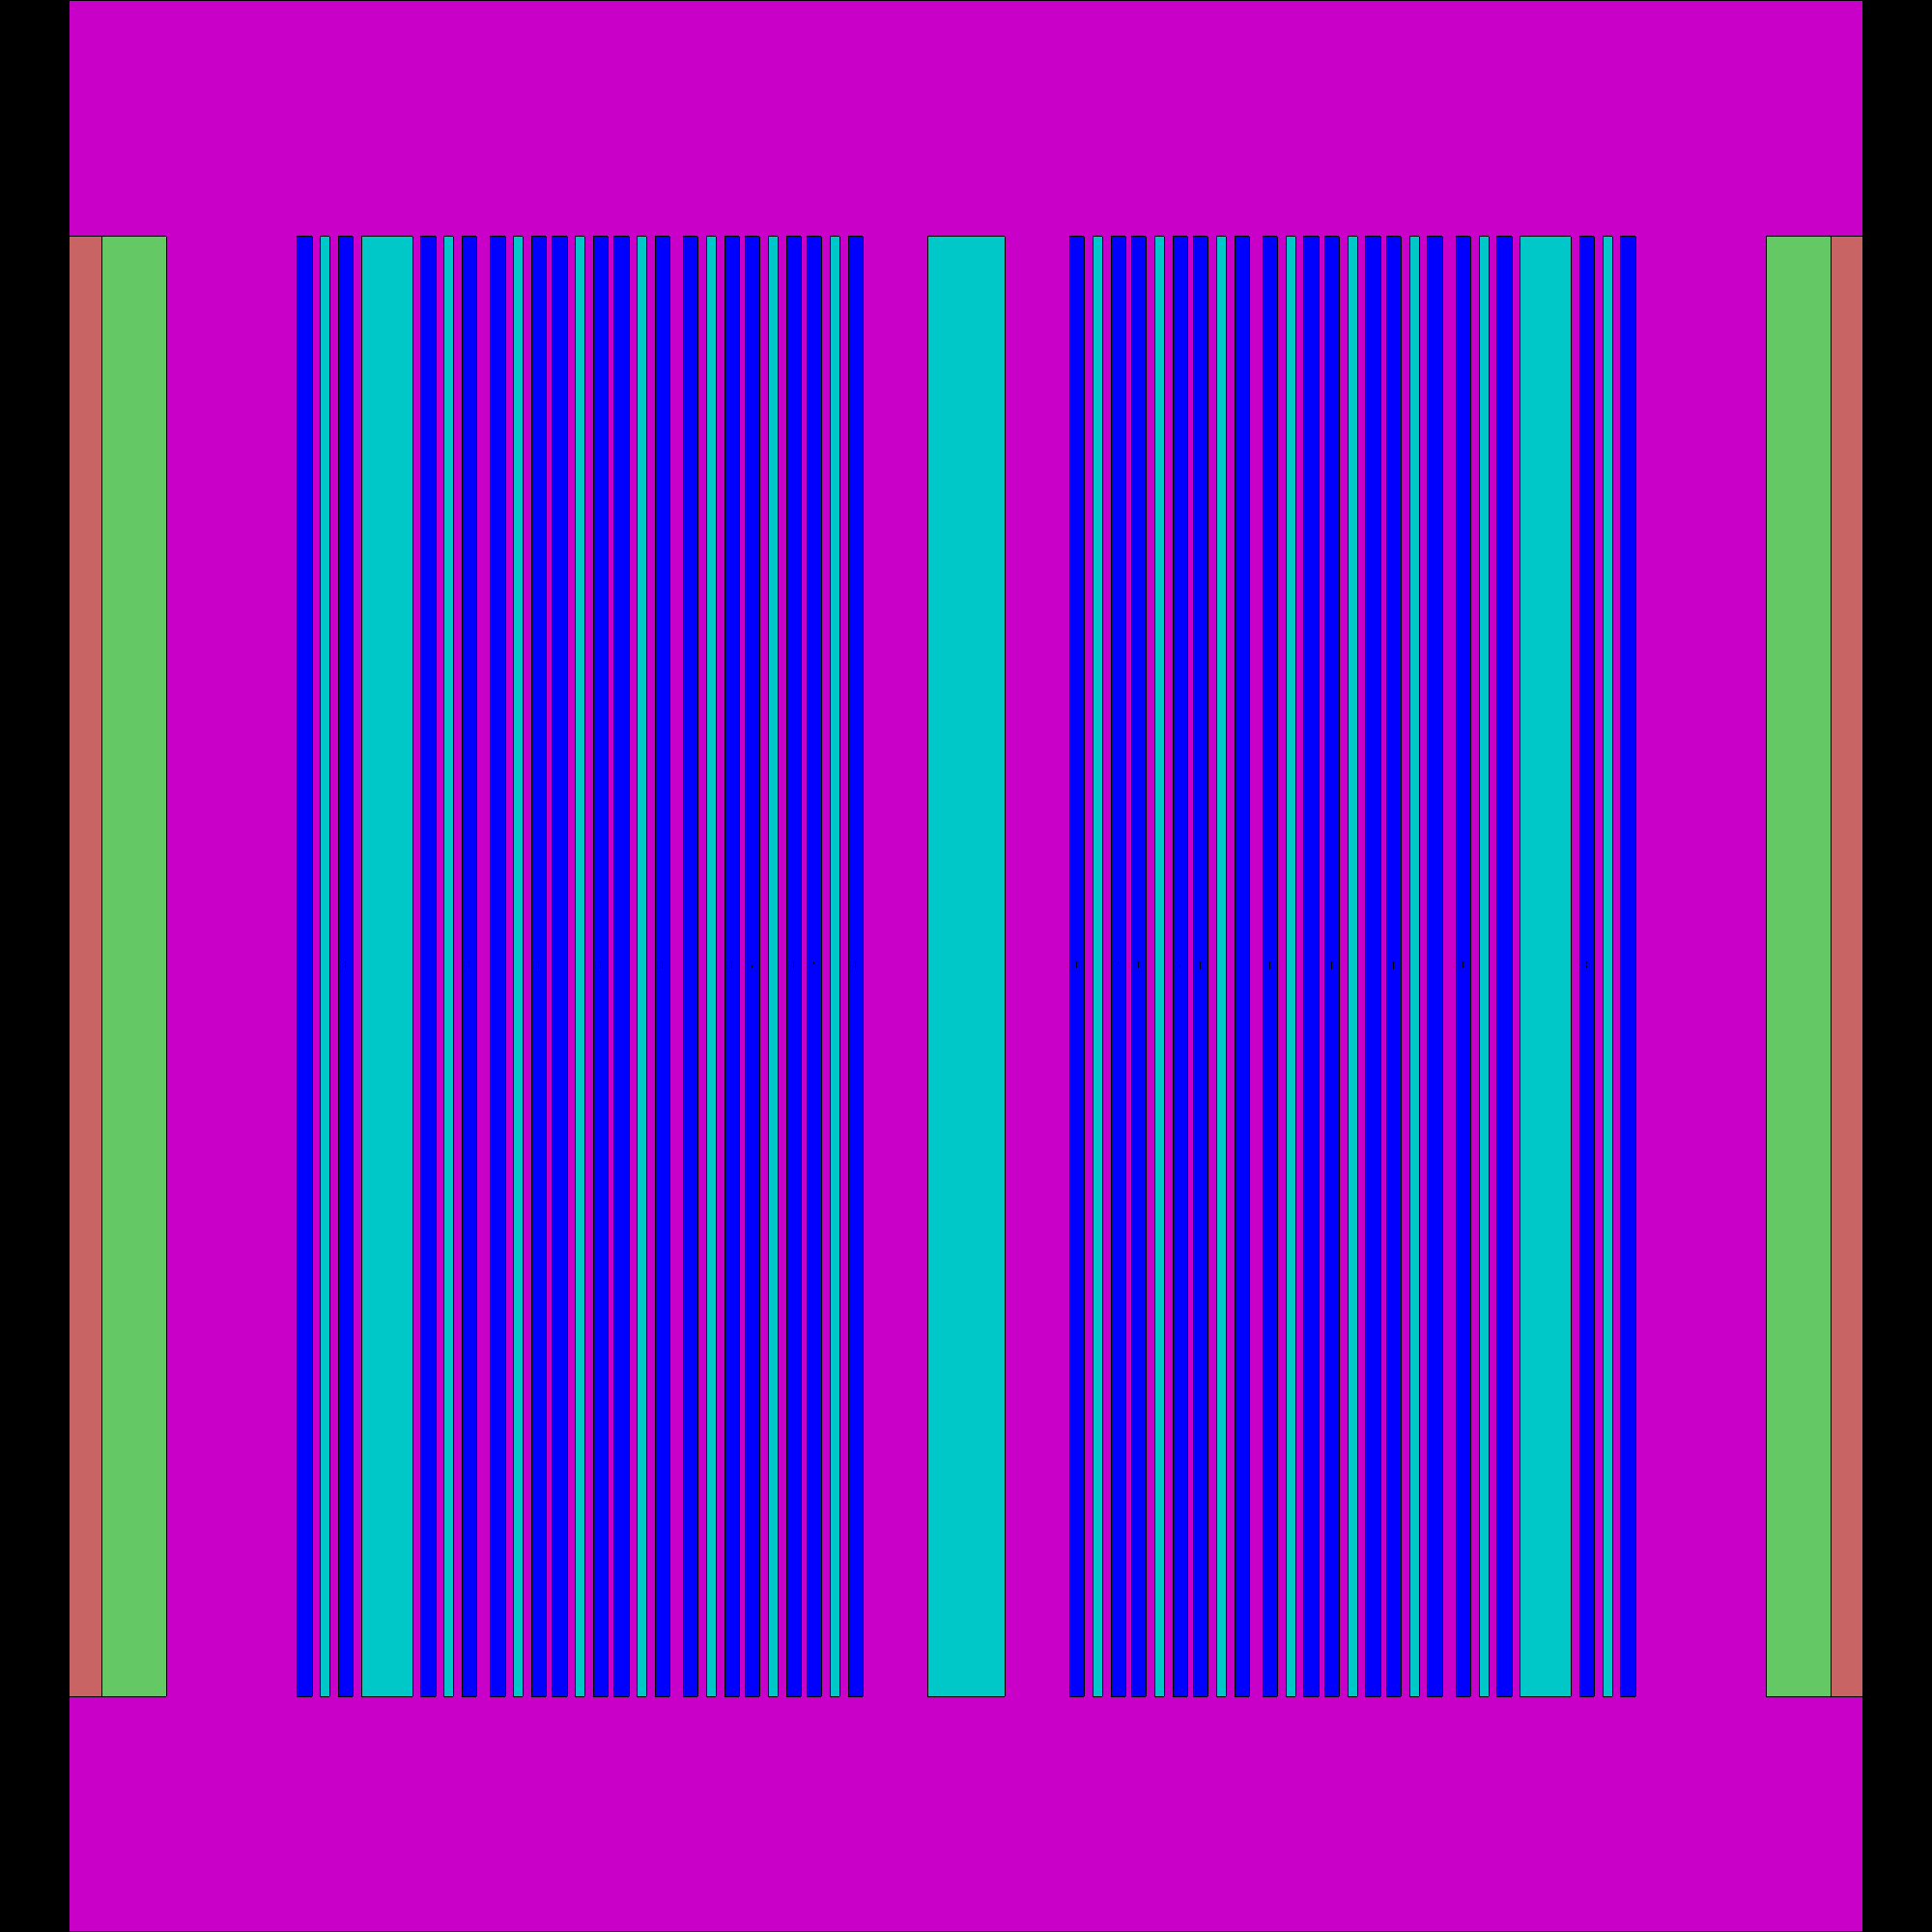
\includegraphics[scale=0.15]{bachmann-mmr_geom3.png}
                \caption{Axial view of the USNC MMR-like model.}
                \label{fig:mmr_axial}
        \end{subfigure}
        \caption{Geometry of USNC MMR-like core model in Serpent. The 
        light blue represents channels helium, dark blue are fuel 
        channels with \gls{FCM} pellets, and the bright pink is graphite in the core.}
        \label{fig:mmr_core}
\end{figure}

For the \gls{MMR}-like model, we modeled depletion of the core across the 
expected 20 year lifetime of the \gls{MMR}, because the core is not 
meant to undergo refueling during those 20 years and the lack of 
fuel movement and replacement in this model aligns with the operational 
core. Depletion is modeled using burnup steps of 2 years. Each burnup step 
was run using 140 active cycles, 75 inactive 
cycles, and 65,000 particles per cycle. 

\subsection{Temperature variations and feedbacks}
The fuel composition burned will affect the population of fission products, 
and consequently the delayed neutron precursors. If substantially different,
the reactor behavior may not be in a safe regime. Consequently, 
one of the goals of this work is to compare the temperature feedback 
coefficients from using the different fuel compositions in each 
reactor. Therefore we varied the fuel, coolant, and moderator temperatures 
between 700, 750, 800, 850, and 900 K to calculate the fuel, coolant, 
moderator, and total temperature feedback coefficients. We assumed a linear 
relationship between 
\keff and temperature to calculate the feedback coefficients. When varying the 
temperatures of each component, we also varied the corresponding material 
density. We calculated the 
density of the UO$_2$ by using the empirical relationship between density and 
temperature defined in \cite{fink_thermophysical_2000}. The calculated 
densities were assumed to hold true for the Sangamon200 fuel. 
We calculated the 
graphite density by linearly extrapolating from the data available in 
\cite{mceligot_thermal_nodate}. We calculated the density of the helium 
by interpolating on the data available in \cite{petersen_properties_nodate}, 
assuming the 3 MPa coolant pressure in the \gls{MMR}-like model as defined 
by \cite{noauthor_usnc_2021} and the 6 MPa inlet pressure in the 
Xe-100-like model as defined in \cite{mulder_overview_2021}. 

\subsection{Fuel compositions}
We used three different \gls{HALEU} compositions for this work: pure 
\gls{HALEU}, and \gls{HALEU} derived from \gls{EBR} and Y-12 \gls{HEU} 
stockpiles. The pure fuel composition assumes that all uranium present is 
either $^{235}$U or $^{238}$U, and at the correct enrichment level for each 
reactor. The \gls{EBR} 
composition is based on the estimated uranium isotopic composition from 
downblending spent fuel from \gls{EBR}, published by \gls{INL} 
\cite{vaden_isotopic_2018}. The Y-12 composition is based on the 
estimated uranium isotopic composition from downblending \gls{HEU} 
stockpiles at the Y-12 National Security Complex \cite{nelson_foreign_2010}.
The published compositions for the \gls{EBR} and Y-12 fuel assume an enrichment 
of 19.75\%, but only the \gls{MMR} requires this level of enrichment. 
Therefore, the uranium isotopic ratios 
published are directly applied for the \gls{MMR} fuel. For the fuel in the 
Xe-100, the isotopic fractions had to be adjusted slightly to match the 
needed enrichment level of 15.5\%. The $^{235}$U fraction was set to match 
the 
enrichment level required, the non-$^{238}$U isotopes were kept in the 
same weight fraction defined in the publications, and the $^{238}$U was 
defined to fill the remainder of the fuel. Therefore, all three fuel compositions for each 
reactor have the same $^{235}$U weight fractions, have non-$^{238}$U weight
fractions that match the published values, and have varying $^{238}$U 
weight fractions for each reactor design. Table \ref{tab:u_comps} defines 
the uranium isotopic composition used 
in each reactor type for each of the \gls{HALEU} compositions. The 
standard for uranium enriched to less than 20\% $^{235}$U, ASTM C1462-21 
\cite{noauthor_standard_2021-1}, sets limits on the the mass of 
$^{232}$U and $^{234}$U relative to the mass of $^{235}$U and the mass of 
$^{236}$U relative to the total mass of the uranium.
The \gls{HALEU} from both \gls{HEU} sources is within the standards, 
using the flexibility of a potential increase in the limit of 
$^{236}$U in the fuel. 

\begin{table}[ht]
        \centering 
        \caption{Atom fraction of uranium isotopes in each \gls{HALEU}
        composition. Uranium fractions are provided, without the oxygen 
        and/or carbon fractions defined. Therefore, the totals in each 
        column for a reactor model do not sum to one.}
        \label{tab:u_comps}
        \begin{tabular}{c c c c}
                \hline
                Isotope & Pure & \gls{EBR} & Y-12 \\
                \hline
                & \multicolumn{3}{c}{Xe-100-like reactor} \\
                $^{232}$U & 0 & 2.40 $\times 10^{-10}$ & 7.27 $\times 10^{-10}$ \\
                $^{233}$U & 0 & 1.78 $\times 10^{-8}$ & 0 \\
                $^{234}$U & 0 & 6.12 $\times 10^{-4}$ & 9.36 $\times 10^{-4}$\\
                $^{235}$U & 5.56 $\times 10^{-2}$ & 5.56 $\times 10^{-2}$ & 5.56 $\times 10^{-2}$\\
                $^{236}$U & 0 & 2.07 $\times 10^{-3}$ & 1.64 $\times 10^{-3}$ \\
                $^{237}$U & 0 & 2.14 $\times 10^{-14}$ & 0 \\
                $^{238}$U & 2.99 $\times 10^{-1}$ & 2.97 $\times 10^{-1}$ & 2.97 $\times 10^{-1}$ \\
                \hline 
                & \multicolumn{3}{c}{MMR-like reactor} \\
                $^{232}$U & 0 & 2.25 $\times 10^{-10}$ & 6.82 $\times 10^{-10}$ \\
                $^{233}$U & 0 & 1.67 $\times 10^{-8}$ & 0 \\
                $^{234}$U & 0 & 5.73 $\times 10^{-4}$ & 8.766 $\times 10^{-4}$ \\
                $^{235}$U & 6.66 $\times 10^{-2}$ & 6.67 $\times 10^{-2}$ & 6.67 $\times 10^{-2}$ \\
                $^{236}$U & 0 & 1.93 $\times 10^{-3}$ & 1.54 $\times 10^{-3}$ \\
                $^{237}$U & 0 & 2.00 $\times 10^{-3}$ & 0 \\
                $^{238}$U & 2.67 $\times 10^{-1}$ & 2.64 $\times 10^{-1}$ & 2.64 $\times 10^{-1}$ \\
                \hline
        \end{tabular}
\end{table}

\section{Results}
The metrics with which we performed our analysis include:
\begin{itemize} 
        \item \keff 
        \item \betaEff
        \item Two-group, spatially dependent neutron flux
        \item Reactivity temperature feedback coefficients for the fuel, coolant, 
              moderator, and the combination of all three.
\end{itemize}

For the Sangamon200, these metrics are only compared in an equilibrium state
of the reactor. For the \gls{MMR}-like reactor these metrics 
are compared at \gls{BOL} (0 MWd/kg burnup), \gls{MOL} (40.52 MWd/kg burnup), 
and \gls{EOL} (81.04 MWd/kg burnup). The two-group structure for 
the neutron flux is based on the default two-group structure in Serpent, 
with the thermal neutrons being between 0-0.625 eV and the fast 
neutrons being above 0.625 eV. Each metric provides a 
measurement of the performance of 
the reactor, such as the materials degradation rate, amount of burnable 
poisons required, control rod worth, and the cycle time. The neutron flux 
informs the materials degradation rate, because a larger neutron flux 
means more damage to the non-fuel materials in the core which may increase 
the frequency of their replacement. The \betaEff affects the control rod 
worth because if too much of the neutron population is born fast then 
the control rods will have less of an effect on controlling the neutron 
chain reaction. The \keff informs the cycle time because the sustainability 
of the neutron chain reaction controls how long a reactor can operate. 
Investigating 
each of these results helps to determine if the impurities 
present in \gls{HALEU} will prevent any of the design criteria of the 
reactors from being met. Results from the simulations are analyzed using 
the serpentTools python package \cite{johnson_serpenttools_2020}. 

\subsection{Xe-100 reactor metric comparisons}
The following four sections report and analyze the results of the 
\gls{EBR} and Y-12 impurities in the Xe-100-like reactor model 
created. The four different results are presented for an 
equilibrium state of the reactor.

\subsubsection{\keff comparison}
Table \ref{tab:xe100_keff} reports the \keff value when using the fuel 
compositions defined in Table \ref{tab:u_comps}. The impure fuels 
result in a \keff 1353-1423 pcm 
greater than the \keff from the pure fuel. All three fuel compositions 
result in a slightly super-critical \keff. The difference in the \keff 
values is more than the error on the values, which means that the 
different fuel compositions result in statistically different \keff 
values for this reactor design. 

\begin{table}[ht]
        \centering 
        \caption{\keff values for the Xe-100-like reactor model for 
        each fuel composition.}
        \label{tab:xe100_keff}
        \begin{tabular}{c c}
                \hline
                Fuel composition & \keff \\
                \hline 
                Pure & 1.06663 $\pm$ 0.00016\\
                \gls{EBR} & 1.08086 $\pm$ 0.00016\\
                Y-12 & 1.08016 $\pm$ 0.00014\\
                \hline                
        \end{tabular}
\end{table}

The uranium isotopes mostly present in 
each of the fuel compositions (weight fraction of at least 1$\times 10^{-3}$)
are $^{234}$U, $^{235}$U, $^{236}$U, and $^{238}$U. The $^{235}$U weight 
fraction is the same in each fuel composition, so the impurities are 
displacing the $^{238}$U in the fuel. $^{234}$U and $^{236}$U have larger 
thermal 
total fission cross sections than $^{238}$U, so their displacement of the
$^{238}$U in the fuel increases the neutron multiplication of the reactor. 
This is supported by the impure fuels leading to a slight increase 
in the thermal fission factor, $\eta$ (1.737 from \gls{EBR} fuel, 1.735 from 
Y-12 fuel, and 1.712 
from pure fuel), which signifies a greater ratio in the number of neutrons
born from fission to the number absorbed in the fuel in the impure 
fuel compositions. The change in $\eta$ is relevant because it is fuel specific, 
but alone it does not define \keff.
Part of the increase in \keff when using the impure fuels is because 
the pebbles modeled are at different burnup steps. Therefore, many of the 
pebbles are already partially burned and the uranium impurities in the fuel 
have already undergone neutron capture reactions and have been transmuted 
into other isotopes that are more fissile. 

The effect of the impure fuels resulting in increased \keff is that more 
control mechanisms may be required to control the chain reaction, or 
to lower the \keff and ensure that the targeted discharge burnup and 
cycle length can be reached. 


\subsubsection{\betaEff comparison}
The \betaEff resulting from the use of each fuel type is reported in 
Table \ref{tab:betaeff_xe100}. The \betaEff from using the pure 
fuel is slightly smaller than the 0.0064 $\beta$ from thermal fissions 
in $^{235}$U because the depletion of some pebbles in the core leads to 
the breeding of $^{239}$Pu from $^{238}$U, which fissions and has 
a smaller \betaEff than $^{235}$U. The \betaEff when using the impure fuels 
is smaller than when using the pure fuel, a difference that is 
statistically significant. The pure fuel results in 
a larger \betaEff than the impure fuels because the other uranium isotopes 
present in the impure fuels breed into fissile material that has 
a smaller \betaEff than $^{235}$U. The depletion modeled to 
obtain compositions of pebbles at different numbers of passes captures 
this breeding of fissile material. The additional fissile material is not 
present in the pure fuel because it's the material that is bred in from 
the uranium impurities. The smaller \betaEff indicates 
that control mechanisms in the reactor will be less effective 
because a larger fraction of the neutron population will be prompt 
neutrons, and there is a smaller time scale on which the neutron 
population can be impacted. 

\begin{table}[ht]
        \centering 
        \caption{\betaEff value from using each fuel type.}
        \label{tab:betaeff_xe100}
        \begin{tabular}{cc}
                \hline
                Fuel type & \betaEff \\
                \hline
                Pure & 0.00617 $\pm$ 0.00003 \\
                \gls{EBR} & 0.00604 $\pm$ 0.00003 \\
                Y-12 & 0.00598 $\pm$ 0.00003 \\
                \hline
        \end{tabular}
\end{table}

\subsubsection{Neutron flux comparison}
Figure \ref{fig:xe100_mg_flux} shows the neutron flux in the 
active region of the core as a function of energy (top) and 
the difference from the pure fuel flux (bottom). The purple 
line in both plots shows the delineation between the fast 
and thermal energy groups in this work (0.625 eV). We used the pre-defined 
SCALE-238 energy group structure in Serpent. 
There is a large peak in the thermal flux around 0.01 MeV. The impure 
\gls{HALEU} compositions have a smaller thermal flux peak 
than the pure fuel, differing on the order of $10^{20}$ 
n/cm$^2$/s. However, at high energies (above 10
MeV) the impure fuels result in a larger flux than the pure 
fuel, differing on the order of $10^{18}$ n/cm$^2$/s. 

\begin{figure}[ht]
        \centering 
        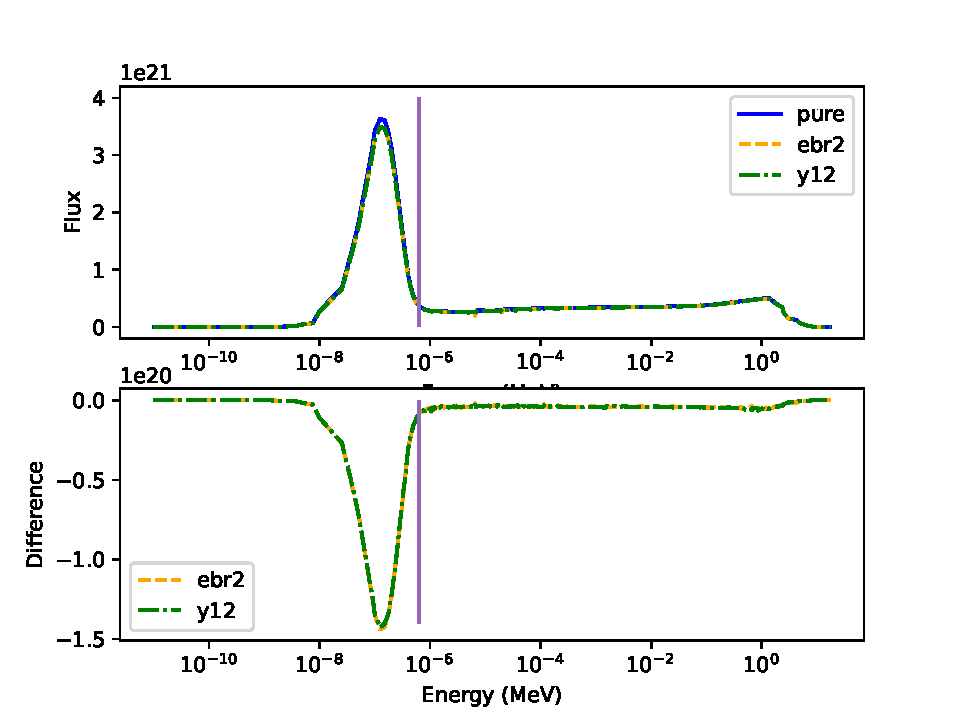
\includegraphics[scale=0.8]{xe100_mg_flux.pdf}
        \caption{238-group flux in the Xe-100-like 
        reactor model in the active region of the core (top). 
        The absolute difference from the flux from 
        the pure \gls{HALEU} fuel (bottom). The purple lines 
        denote the delineation of the thermal and fast 
        energy groups used in this work.}
        \label{fig:xe100_mg_flux}
\end{figure}

Figures \ref{fig:xe100_thermal_radial}-\ref{fig:xe100_fast_axial} show 
thermal and fast fluxes in the reactor core axially and radially. 
The thermal radial flux spectra from all three \gls{HALEU} compositions 
(Figure \ref{fig:xe100_thermal_radial})
show peaks at the edge of the core resulting from the graphite moderator 
around the core. The middle of the core exhibits a notable 
difference in the neutron flux between the impure and pure fuel 
compositions. The impure fuel compositions result in a slightly 
lower flux than the pure fuel, which is consistent with the 
results shown in Figure \ref{fig:xe100_mg_flux}. 
However, the smaller thermal flux is in contrast to the larger 
\keff from the impure fuels. This difference in trend of the \keff and 
the neutron flux suggests that the impurities in the fuel lead to 
more neutrons born from fissions but the neutrons travel a shorter 
distance in the core before being absorbed. 

\begin{figure}[ht]
        \centering 
        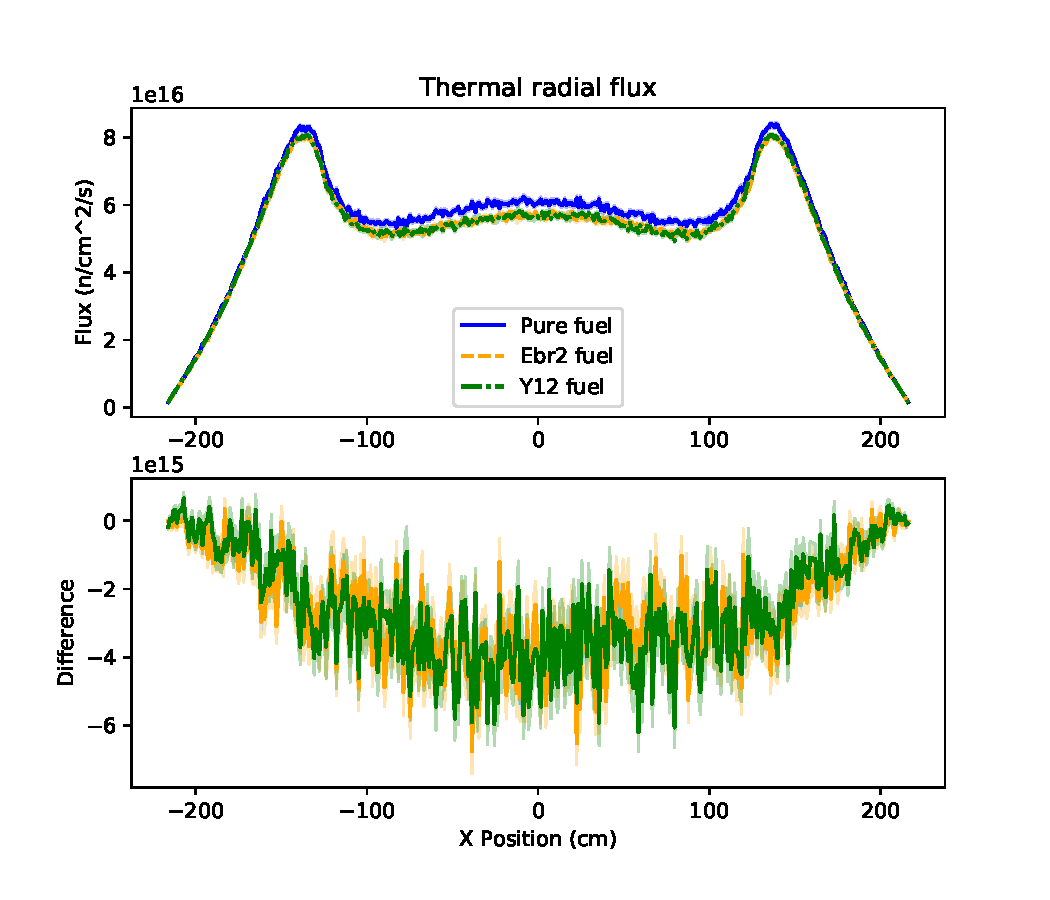
\includegraphics[scale=0.8]{xe100_thermal_radial.pdf}
        \caption{Thermal flux (below 0.625 eV) in the Xe-100-like Sangamon200 
        reactor model in the radial direction, across the 
        x-axis (top). The absolute difference from the flux from 
        the pure \gls{HALEU} fuel with 1$\sigma$ error shown by 
        the shading (bottom).}
        \label{fig:xe100_thermal_radial}
\end{figure}

$^{238}$U has the largest difference between the total and total 
fission cross sections of the uranium isotopes considered for this model. 
So by replacing the U-238 with other isotopes the flux should 
increase from the larger fission to total ratio because the other isotopes 
are more likely to have fission reactions and produce neutrons.
Another factor to consider in this analysis is that this core is not 
comprised of exclusively fresh fuel. 
The use of burned pebbles in this model affects the flux because the 
fission yield curves are different for each fissile isotope. If some 
of the fissions are occurring from reactions in $^{233}$U compared with 
$^{235}$U, than the fission products present in the partially 
burned pebbles will be different which affects the neutron reaction 
rate densities in the core. Also, the even uranium isotopes 
(e.g., $^{234}$U) have relatively small fission cross sections, 
so they're still more likely to absorb a neutron than to fission. 

Figure \ref{fig:xe100_fast_radial} shows the fast radial flux from 
each \gls{HALEU} composition in this work. The fast fluxes do not 
exhibit the same peaks in the reflector as the thermal flux 
because of the neutron energy difference. The peak magnitude of 
the fast flux is slightly 
larger than the thermal flux, indicating that more of the neutrons 
in the core are at higher energies. The impure fuels also result in a 
slightly lower flux in the middle of the core, compared with the  
flux from the pure fuel. The differences in the fast fluxes are on similar 
order of magnitude to the differences in the thermal fluxes (about $\pm$ 
2-4 $\times 10^{15}$ n/cm$^2$/s), but the fast fluxes are larger than 
the thermal fluxes. Therefore, the impurities result in a smaller overall
relative difference in the fast flux than they do in the thermal 
flux. These results are all consistent with the multi-group flux results. 
The total area under the curve in the fast region of Figure 
\ref{fig:xe100_mg_flux} is greater than the area under the curve 
in the thermal region of that figure, indicating that more neutrons 
are in the fast energy range. Also, the increase in flux above 
10 MeV from the impure fuels is less than the decrease in the flux 
from the impure fuels between 0.0625 eV--10 MeV, which is why 
Figure \ref{fig:xe100_fast_radial} shows that the impure 
fuels result in a smaller flux. 

\begin{figure}[ht]
        \centering 
        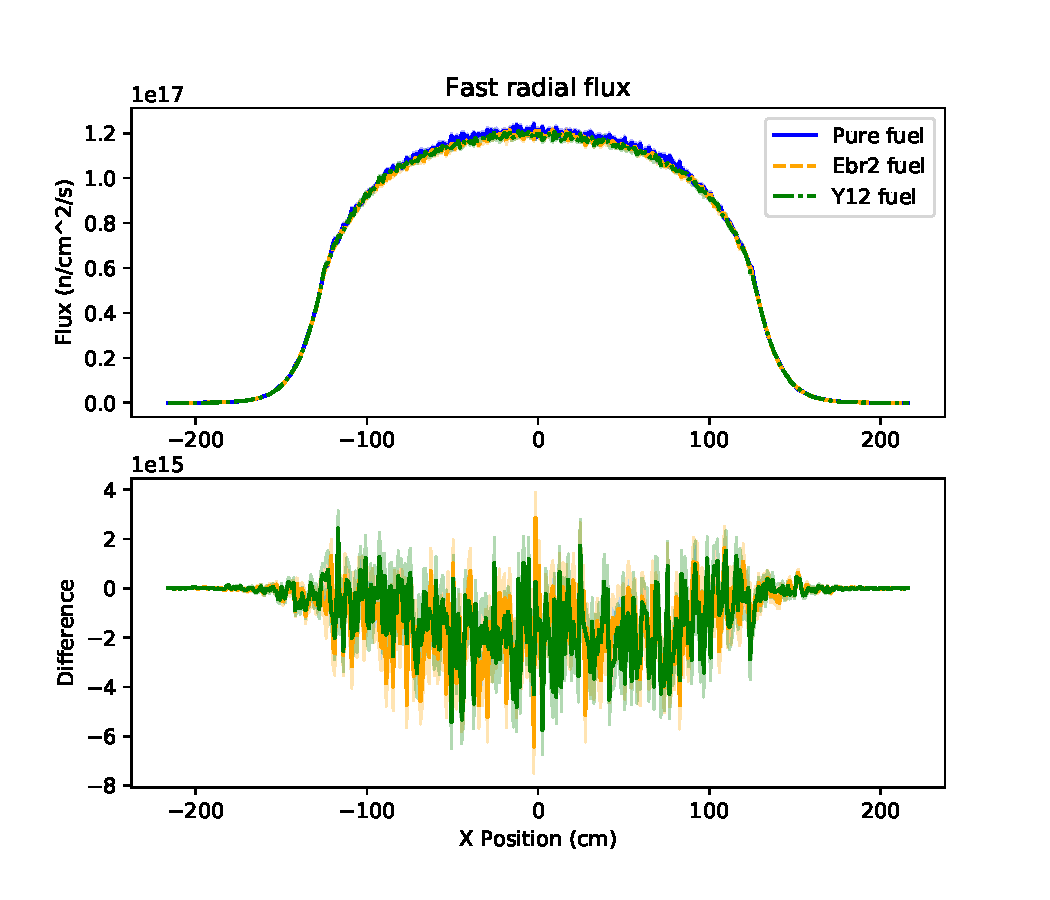
\includegraphics[scale=0.8]{xe100_fast_radial.pdf}
        \caption{Fast flux (above 0.625 eV) in the Xe-100-like Sangamon200 
        reactor model in the radial direction, across the 
        x-axis (top). The absolute difference from the flux from 
        the pure \gls{HALEU} fuel with 1$\sigma$ error shown by 
        the shading (bottom).}
        \label{fig:xe100_fast_radial}
\end{figure}


The thermal axial flux (Figure \ref{fig:xe100_thermal_axial}) shows 
similar results to the thermal radial flux and the multi-group flux. 
There is a small bump in the 
flux at the top and bottom of the core because of the graphite reflector.
Additionally, the pure fuel results in a larger flux than 
the impure fuels. The two impure fuel compositions result in very 
similar fluxes. The flux differences between the fuel compositions is 
larger in the bottom of the core, causing flux asymmetry in the core. The
pure fuel resulting in a larger thermal flux than the impure fuel is consistent with the larger \betaEff 
from the pure fuel. Delayed neutrons are born in the thermal energy range, 
so a larger \betaEff means that a larger fraction of the neutrons are 
born in the thermal energy range. 

\begin{figure}[ht]
        \centering 
        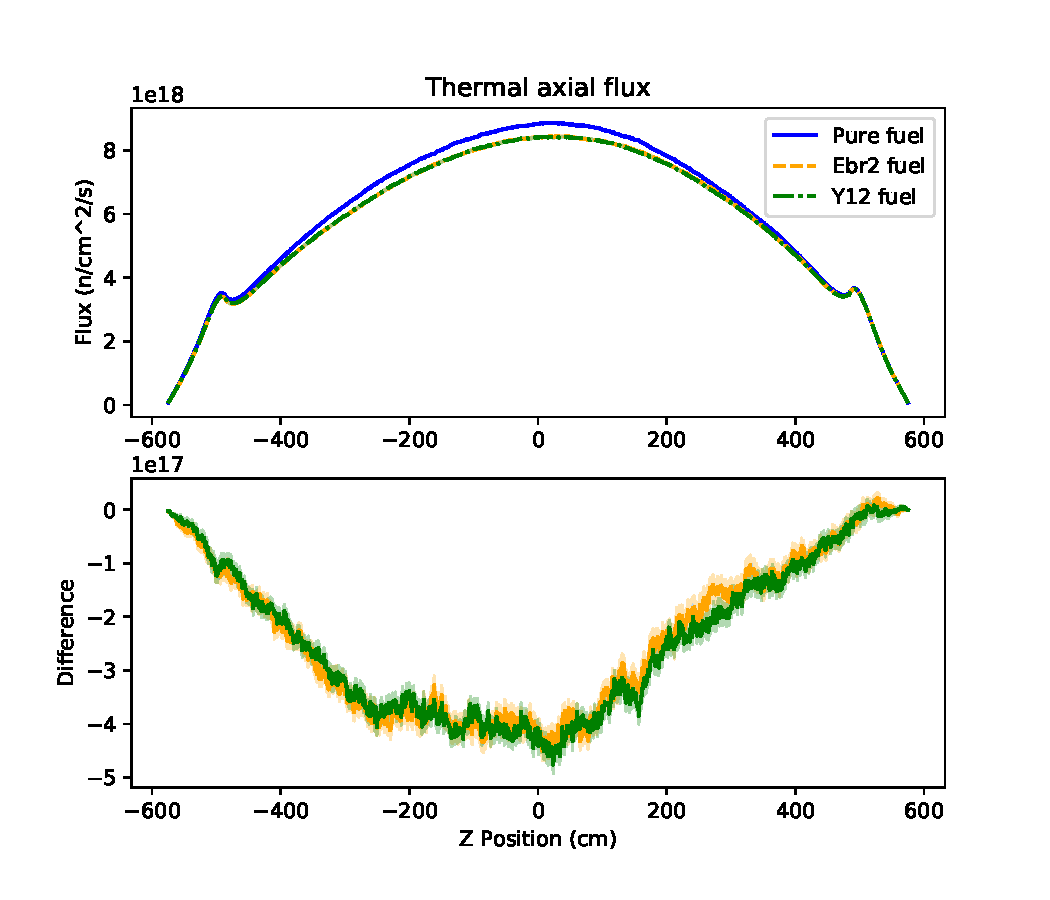
\includegraphics[scale=0.8]{xe100_thermal_axial.pdf}
        \caption{Thermal flux (below 0.625 eV) in the Xe-100-like Sangamon200 
        reactor model in the axial direction (top). The absolute 
        difference from the flux from 
        the pure \gls{HALEU} fuel with 1$\sigma$ error shown by 
        the shading (bottom). 0 cm is the midpoint of the core.}
        \label{fig:xe100_thermal_axial}
\end{figure}

The asymmetry in the differences in 
the fluxes is primarily a result of the pebble placement. The 
pebbles are all evenly spaced around the core, and there are an equal 
number of pebbles at each integer pass number. However, the pebbles of 
each pass number are not evenly distributed across the core. 
This was confirmed by shuffling the locations of the pebbles at each 
pass number when using the Y-12 fuel: fresh pebbles switched with most 
burnt, single pass pebbles switched with pebbles that have gone through 
all but one passes, etc. The thermal axial flux when shuffling the Y-12 
fuel  
pebble locations (Figure \ref{fig:xe100_pebble_shuffle}) shows that 
changes the symmetry of the difference. Therefore, some of the difference 
in the neutron flux is a result of the placement of the pebbles, and 
the differences in isotopic compositions from burning the different 
fuel compositions. However, shuffling the pebbles when using the Y-12 
\gls{HALEU} composition still resulted in a smaller flux than the 
pure fuel. Therefore, the flux depression is a function of the 
\gls{HALEU} composition and not the pebble placement.

\begin{figure}[ht]
        \centering 
        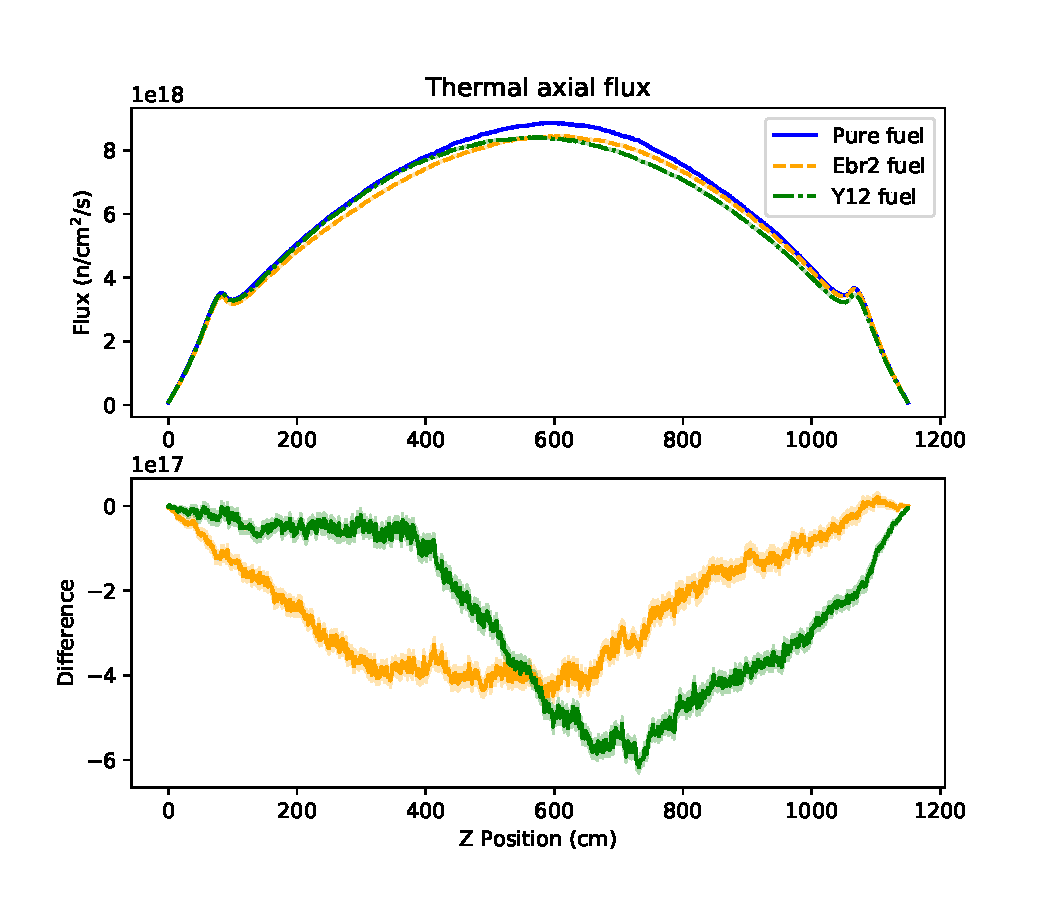
\includegraphics[scale=0.8]{xe100_shuffled_thermal_axial.pdf}
        \caption{Thermal flux (below 0.625 eV) in the Xe-100-like Sangamon200 
        reactor model in the axial direction when the locations of 
        the pebbles are shuffled when using the Y-12 fuel composition
        (top). The absolute difference from the flux from 
        the pure \gls{HALEU} fuel with 1$\sigma$ error shown by 
        the shading (bottom).}
        \label{fig:xe100_pebble_shuffle}
\end{figure}

The fast axial flux (Figure \ref{fig:xe100_fast_axial}) shows a smaller 
difference in the flux magnitudes between the different fuel compositions 
than the thermal axial fluxes. The 
impure fuels result in similar fluxes, consistent to observations in 
the thermal axial flux. The largest flux difference between the pure 
and impure fuels is also in the bottom of the core. However, unlike 
in the thermal axial flux, impure fuels result in a slightly larger 
flux than the pure fuel in the top of the core. The axial asymmetry in 
the difference between the fluxes is consistent with the differences in 
the thermal axial fluxes because of the effect of pebble location 
and the different compositions in partially burned fuel. 

\begin{figure}[ht]
        \centering 
        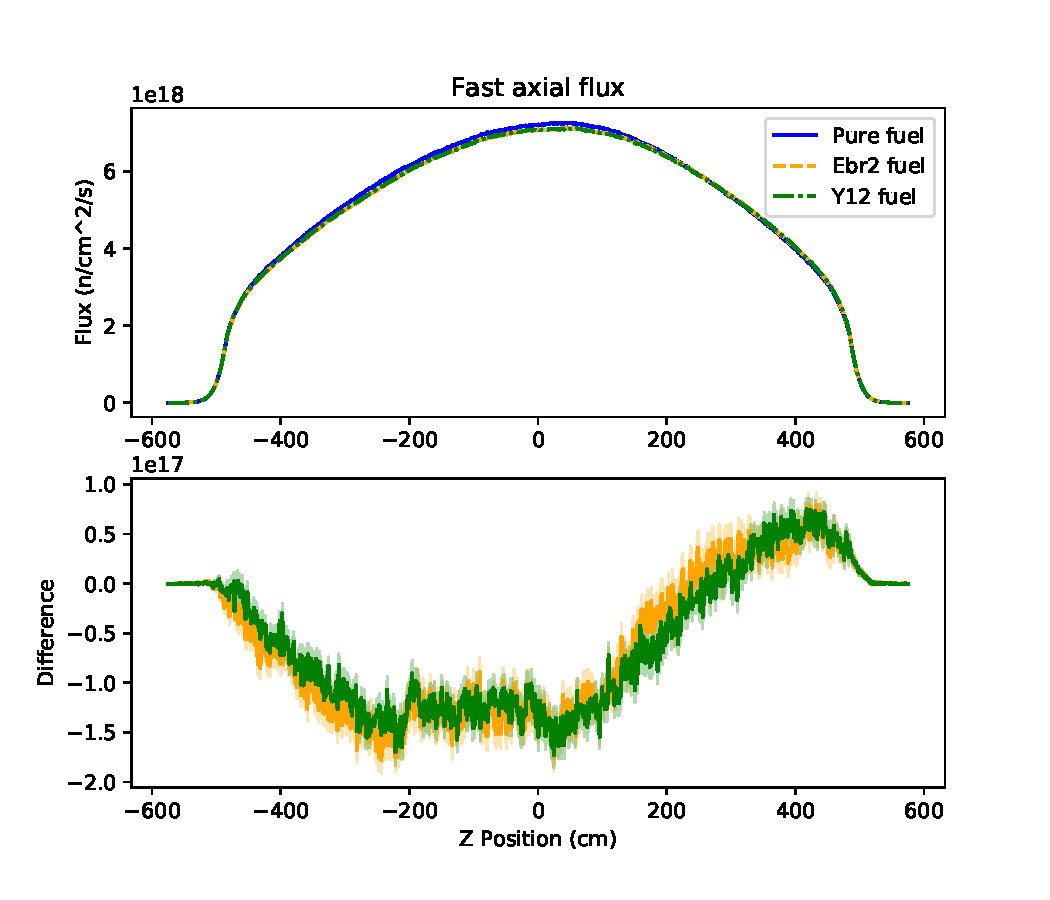
\includegraphics[scale=0.8]{xe100_fast_axial.pdf}
        \caption{Fast flux (above 0.625 eV) in the Xe-100-like Sangamon200 
        reactor model in the axial direction (top). The absolute 
        difference from the flux from 
        the pure \gls{HALEU} fuel with 1$\sigma$ error shown by 
        the shading (bottom).}
        \label{fig:xe100_fast_axial}
\end{figure}

The fluxes from this reactor model are about three orders of 
magnitudes larger than the results from the modeling of the 
Xe-100 done by Mulder and 
Boyes \cite{mulder_neutronics_2020}. Part of this difference comes 
from the ranges used for each energy group. Mulder and Boyes used 
a definition of greater than 0.1 MeV for the fast energy group and 
less than 1.86 eV for the thermal energy group. This work applies a 
definition of greater than 0.625 eV and less then 0.625 eV for fast 
and thermal neutrons, respectively. Therefore, the definitions used by 
Mulder and Boyes does not include all possible neutron energies 
while the definition used in this work does, leading to some of the 
differences between the fluxes. 
The other difference  comes from the detector 
definitions in the inputs. For this work, the radial detector 
was defined across the x- and y-axes and the axial detector was defined 
across the z-direction. The flux in a detector in Serpent is integrated 
across the volume of the core \cite{leppanen_serpent_2013}. Therefore, 
the flux across any axes not included in the mesh for a detector is 
summed across those axes. This is the primary reason why the flux is 
orders of magnitude different between the two models. 

\subsubsection{Reactivity feedback coefficient comparison}
Table \ref{tab:coeff_xe100} reports the reactivity feedback 
coefficients for each material type in the Xe-100-like reactor model. 
All of the coefficients are negative: this is a positive feature of 
this reactor so that reactivity naturally decreases as temperature 
increases. 

\begin{table}[ht]
        \centering
        \caption{Reactivity temperature feedback coefficients for 
        each material type in the Xe-100-like model for each fuel 
        type.}
        \label{tab:coeff_xe100}
        \begin{tabular}{c c c c c}
            \hline 
            & \multicolumn{4}{c}{Material feedback coefficient (pcm/K)} \\
            Fuel Type & Fuel & Coolant & Moderator & Total \\
            \hline
            Pure & -3.875 $\pm$ 0.094 & -0.044 $\pm$ 0.112 & -0.071 $\pm$ 0.459 & -4.216 $\pm$ 0.502\\
            \gls{EBR} & -3.759 $\pm$ 0.138 & -0.433 $\pm$ 0.048 & -0.708 $\pm$ 0.404 & -4.817 $\pm$ 0.438\\
            Y-12 & -3.797 $\pm$ 0.157 & -0.351 $\pm$ 0.092 & -0.728 $\pm$ 0.469 & -4.700 $\pm$ 0.349\\
            \hline

        \end{tabular}
\end{table}

The fuel reactivity feedback coefficient from the pure fuel is more 
negative than the values from the impure fuels, with the \gls{EBR} fuel 
resulting in the least negative fuel feedback coefficient. However, all of 
the values are negative, and are within error of each other. Therefore, 
one cannot conclude that the fuel composition significantly affects this 
metric. 

For the other three reactivity feedback coefficients, the impure fuels 
result in coefficients that are more negative than the values from 
the pure fuel. The coolant feedback coefficient values are outside 
of the reported error (pure compared with a non-pure fuel), but the 
values of the other two material coefficients are all within error of 
each other. The significant impact on the coolant reactivity feedback 
coefficient suggests that the impurities in the fuel cause a larger 
flux near the single resonance in the total cross section for helium,
resulting in the greater impact from changing this material temperature. 
However based on the values of each material feedback coefficient, 
the coolant temperature has a much smaller effect and impact on the 
total feedback coefficient than the other materials. 

The work by Mulder and Boyes \cite{mulder_neutronics_2020}, reported 
the reactivity coefficients reported in Table \ref{tab:mulder_coeffs}
for temperatures between 100-900
\textdegree C. The feedback coefficients are within the ranges reported 
by Mulder and Boyes, despite the differences in the reactor models used.
The consistency between the feedback coefficient values from the impure 
fuels in this work and the values reported by Mulder and Boyes suggests that 
the impurities in the fuel do not greatly impact this reactor operation 
metric.  

\begin{table}[ht]
        \centering 
        \caption{Reactivity temperature feedback coefficient maximum and 
        minimum values reported by Mulder and Boyes for the Xe-100 between 
        100-900 \textdegree C \protect\cite{mulder_neutronics_2020}.}
        \label{tab:mulder_coeffs}
        \begin{tabular}{c c c}
                \hline 
                Reactivity coefficient & Minimum ($\Delta$ \keff/\textdegree C) 
                & Maximum ($\Delta$ \keff/\textdegree C)\\
                \hline
                Fuel Doppler & -5.6e-5  & -3.2e-5 \\
                Moderator & -4.2e-5 & -0.4e-5 \\
                Total & -6.1e-5 & -2.0e-5\\
                \hline

        \end{tabular}
\end{table}

\subsection{MMR reactor}
The following four sections report and analyze the results of the 
\gls{EBR} and Y-12 impurities in the \gls{MMR}-like reactor model 
created. The four different results are presented for three different 
burnup steps during the reactor operation: \gls{BOL} (0 MWd/kgU),
\gls{MOL} (40.52 MWd/kgU), and \gls{EOL} (81.04 MWd/kgU). 

\subsubsection{\keff comparison}
Table \ref{tab:mmr_keff} reports the \keff value of the \gls{MMR} at the 
different burnup steps using each fuel composition. At each burnup step, 
using the impure fuel compositions results in a \keff 712-1344 pcm 
smaller than the \keff when using the pure fuel. The difference in \keff 
from the different fuel compositions decreases with burnup because of 
the depletion of the uranium, which includes burning of the parasitic 
uranium isotopes. The impure fuel resulting in a lower \keff 
than the pure fuel is the opposite 
effect of that observed in the Xe-100-like model. The change in the trend 
is because in this reactor the fuel is more homogeneous than in 
the Xe-100-like model. In the Xe-100-like model, the pebbles are modeled 
at different burnup stages, while in this model all of the fuel is at the 
same burnup step. All of the fuel in this model is unburned in the 
first burnup step, meaning that the impurities have a more significant 
effect on the neutron population because the impurities are a larger fraction 
of the uranium in the core than in the Xe-100-like model.

\begin{table}[ht]
        \centering
        \caption{\keff in the \gls{MMR}-like model at select burnup 
        steps and different \gls{HALEU} compositions.}
        \label{tab:mmr_keff}
        \begin{tabular}{c c c c}
                \hline 
                & \multicolumn{3}{c}{Burnup step}\\
                Fuel Type & \gls{BOL} & \gls{MOL} & \gls{EOL} \\
                \hline 
                Pure & 1.33797 $\pm$ 0.00027 & 1.18048 $\pm$ 0.00025 & 1.05535$\pm$000024\\
                \gls{EBR} & 1.32609 $\pm$0.00028 & 1.17148 $\pm$ 0.00027 & 1.04792 $\pm$ 0.00025 \\
                Y-12 & 1.32453$\pm$0.00029 & 1.17051$\pm$0.00027 & 1.04823$\pm$0.0024\\
                \hline
                
        \end{tabular}
\end{table}

The effect of of the impurities on this reactor model are significant on the 
\keff; the differences exceed the error on the values. However, 
even at the last burnup step the \keff is still above 1. Therefore the 
effect of the impurities 
is not great enough to cause the reactor to reach a subcritical state 
during its operation. The super-critical \keff throughout the duration 
of the burn cycle suggests that the lifetime of the reactor will not be 
affected by the impurities in the fuel.

\subsubsection{\betaEff comparison}
Table \ref{tab:mmr_betaeff} reports the \betaEff values when using 
each fuel composition at the different burnup steps. For all three 
fuel compositions, the \betaEff decreases with increasing burnup. This 
is consistent with the depletion of the $^{235}$U in the core and 
an increase in the number of fissions happening in isotopes
that have a lower \betaEff than $^{235}$U, such as $^{239}$Pu. 
The \betaEff values at \gls{BOL} are slightly larger 
than the expected 0.0064 value of $\beta$ for thermal fissions in $^{235}$U
or the \betaEff of a typical \gls{PWR}. The consistency of the \betaEff 
larger than 0.0064 at \gls{BOL} across the three \gls{HALEU} compositions 
is a result of the smaller geometry of this core compared with a 
\gls{PWR} core, and not an effect of the fuel compositions. 
The small size of the core and higher enrichment cause an 
increase in the probability of non-leakage of fast neutrons to 
dominate the decrease of the fast fission factor, compared with a \gls{PWR}. 

\begin{table}[ht]
        \centering
        \caption{\betaEff value in the \gls{MMR}-like model at 
        select burnup steps.}
        \label{tab:mmr_betaeff}
        \begin{tabular}{c c c c}
                \hline 
                 & \multicolumn{3}{c}{Burnup step}\\
                Fuel & \gls{BOL} & \gls{MOL} & \gls{EOL}\\
                \hline 
                Pure & 0.00669 $\pm$ 0.00004 & 0.00586 $\pm$ 0.00004 & 0.00548 $\pm$ 0.00003\\
                \gls{EBR} & 0.00663 $\pm$ 0.00003 & 0.00591 $\pm$ 0.00003 & 0.00542 $\pm$ 0.00003\\
                Y-12 & 0.00665 $\pm$ 0.00004 &  0.00598 $\pm$ 0.00004& 0.00553 $\pm$ 0.00003\\
                \hline 

        \end{tabular}
\end{table}

Each of the fuel compositions result in different \betaEff values at 
each burnup step. However, almost all of the values from the impure 
fuels are within error of the value from the pure fuel. Therefore, the 
fuel impurities do not lead to any significant changes in the 
\betaEff. Additionally, the impure fuel compositions do not lead to 
a consistent change in \betaEff between burnup steps. Based on 
these results, the control rod worth and response time will be 
comparable when using any of these three \gls{HALEU} compositions.

\subsubsection{Neutron flux comparison}
Figure \ref{fig:mmr_energy_spectrum} shows the flux in the active 
region of the core as a function of energy (top) and the difference between 
the flux from the pure fuel and each of the impure fuels (bottom). This 
data was 
calculated using the pre-defined SCALE-238 energy group structure in Serpent,
with the plotted flux of each group normalized by lethargy. The purple 
line in both plots in the figure shows the delineation between the fast and 
thermal energy groups (0.625 eV). This figure shows that the difference between 
the fluxes is small compared with the magnitude of the flux ( two orders 
of magnitude different), especially in 
the thermal group (left of the purple line). The difference between the 
fluxes is larger in the epithermal and fast regions, such that the largest 
difference in the peak around 1 MeV. The differences 
in the flux from the pure fuel and the flux from each of the impure 
fuels is larger in the fast energy group than in the thermal energy group.

\begin{figure}
        \centering
        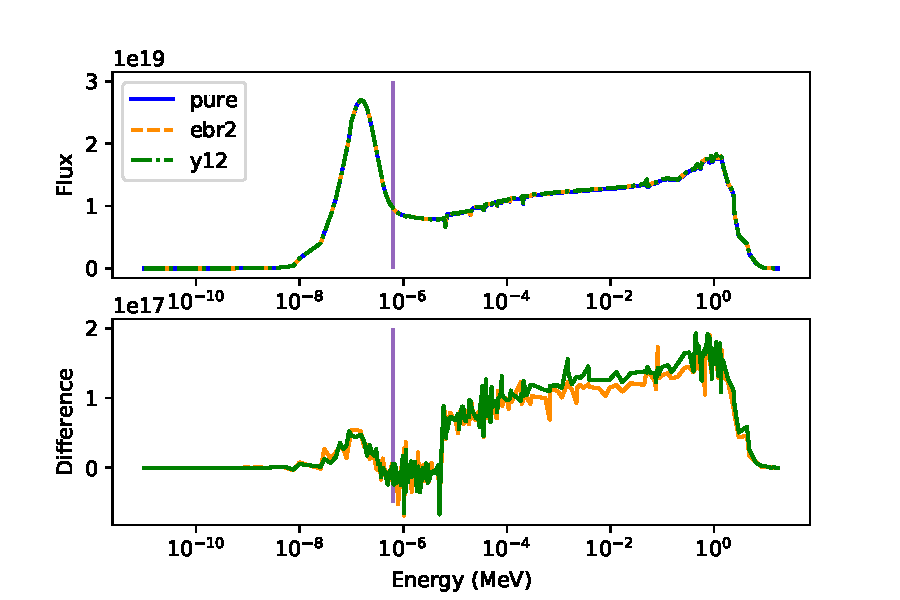
\includegraphics{mmr_energy_spectrum.pdf}
        \caption{Top: Flux energy spectrum for each fuel composition at a 
        burnup of 0 MWd/kgU in the active region of the core. The 
        purple line shows the delineation between the fast and thermal 
        neutron energy groups used in other results of this work.
        Bottom: Difference between the flux from the pure fuel and each 
        of the impure fuels in each energy group. The purple line shows the 
        delineation between the fast and thermal energy groups (0.625 eV). }
        \label{fig:mmr_energy_spectrum}
\end{figure}

Figures \ref{fig:mmr_bol}, \ref{fig:mmr_mc}, and \ref{fig:mmr_eol} show 
the neutron flux in the thermal and fast energy ranges in the radial and axial 
direction for the \gls{BOL}, \gls{MOL}, and \gls{EOL} burnup steps, 
respectively. The radial fluxes are taken 
across the middle of the core in the y-direction, which means the flux 
is taken across the plane with three coolant channels in Figure 
\ref{fig:mmr_radial}. The effects of the coolant channels can be observed 
in the oscillations of the radial fluxes at each burnup step. The axial 
flux is taken along the z-axis, with the 
x- and y-directions collapsed. As a result, the axial flux includes 
radially averaged behavior. 

The radial flux at \gls{BOL} (Figures \ref{fig:mmr_thermal_radial_bol} and 
\ref{fig:mmr_fast_radial_bol}) show that the thermal flux peaks in the 
control rod channels and the fast flux has a trough in these regions. 
Conversely, the thermal flux has a trough in the areas closest to the fuel 
channels and the fast flux has a peak in these areas. These features occur 
because neutrons from fission in the fuel are born in the fast energy 
range, but are thermalized as they travel through the graphite towards 
the coolant channels. 
The greatest difference in the 
fluxes between the fuel compositions is in the areas of the core close 
to the fuel pellets, where the thermal flux troughs and the fast flux 
peaks. This result is consistent with only the fuel 
composition changing between each core model, as the different fuel 
compositions would lead to different energy spectrums for the neutrons 
born form fission and thermalizing in the graphite around the fuel channels.
The fast flux along this axis is larger than the thermal flux, which is 
consistent with the observation of the active-core flux as a function of 
energy. Similar to the neutron flux in the Xe-100-like model, the 
impure fuels result in similar variations from the flux when 
using the pure fuel at this burnup step.

\begin{figure}[h!]
        \centering
        \begin{subfigure}[b]{0.48\textwidth}
            \centering
            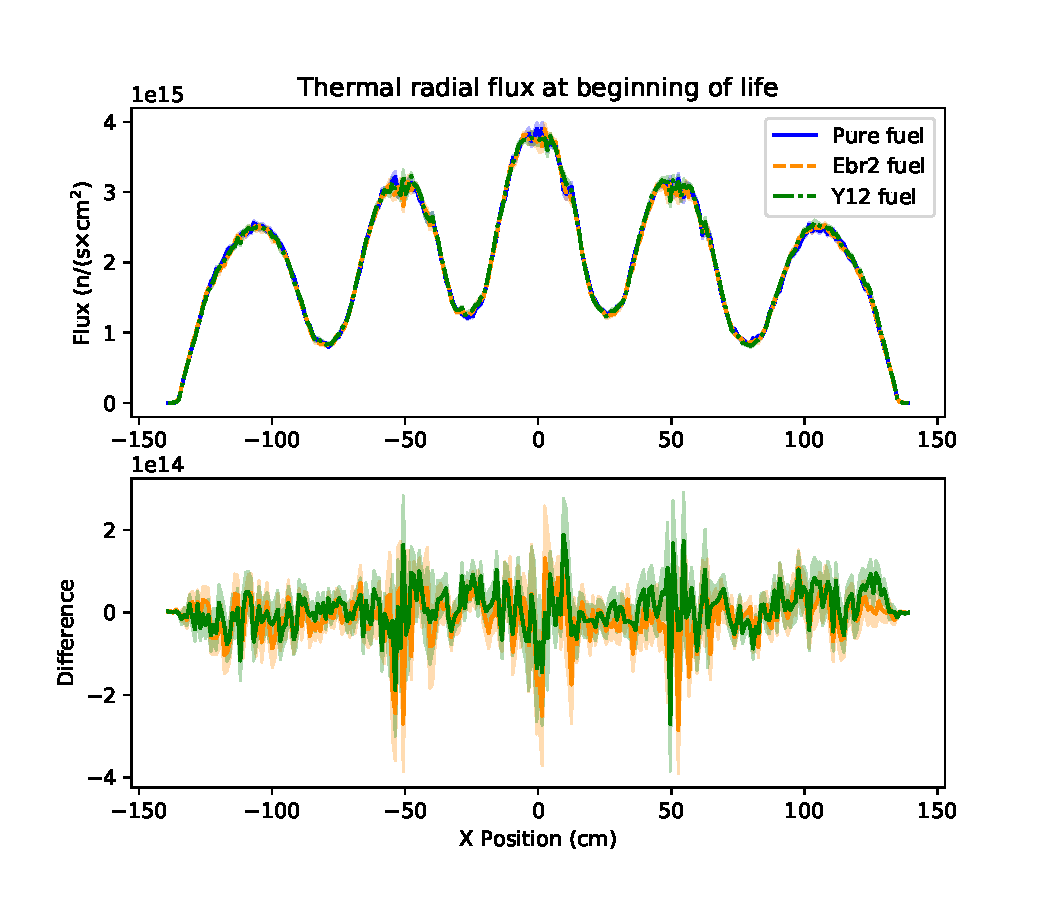
\includegraphics[width=\textwidth]{mmr_thermal_radial_bol.pdf}
            \caption{Thermal radial flux in the \gls{MMR}-like reactor.}
            \label{fig:mmr_thermal_radial_bol}
        \end{subfigure}
        \hfill
        \begin{subfigure}[b]{0.48\textwidth}
            \centering
            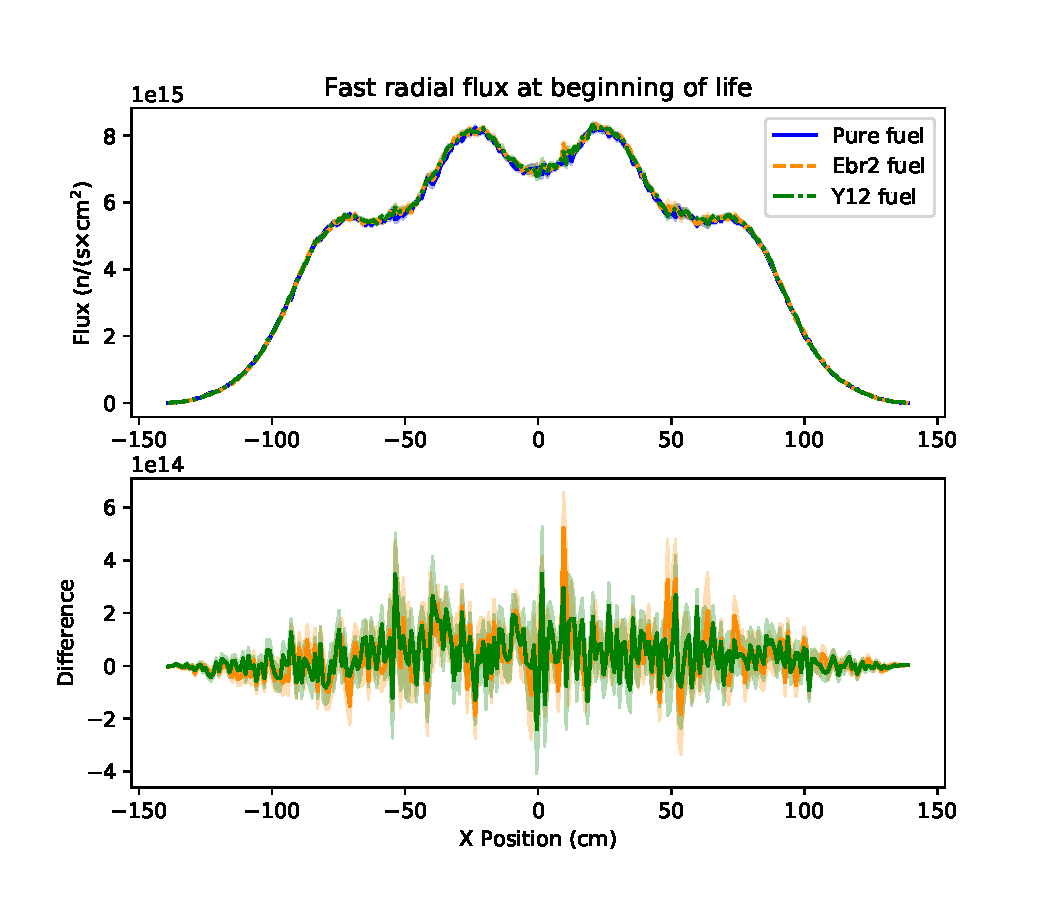
\includegraphics[width=\textwidth]{mmr_fast_radial_bol.pdf}
            \caption{Fast radial flux in the \gls{MMR}-like reactor.}
            \label{fig:mmr_fast_radial_bol}
        \end{subfigure}
        \hfill            
        \begin{subfigure}[b]{0.48\textwidth}
            \centering
            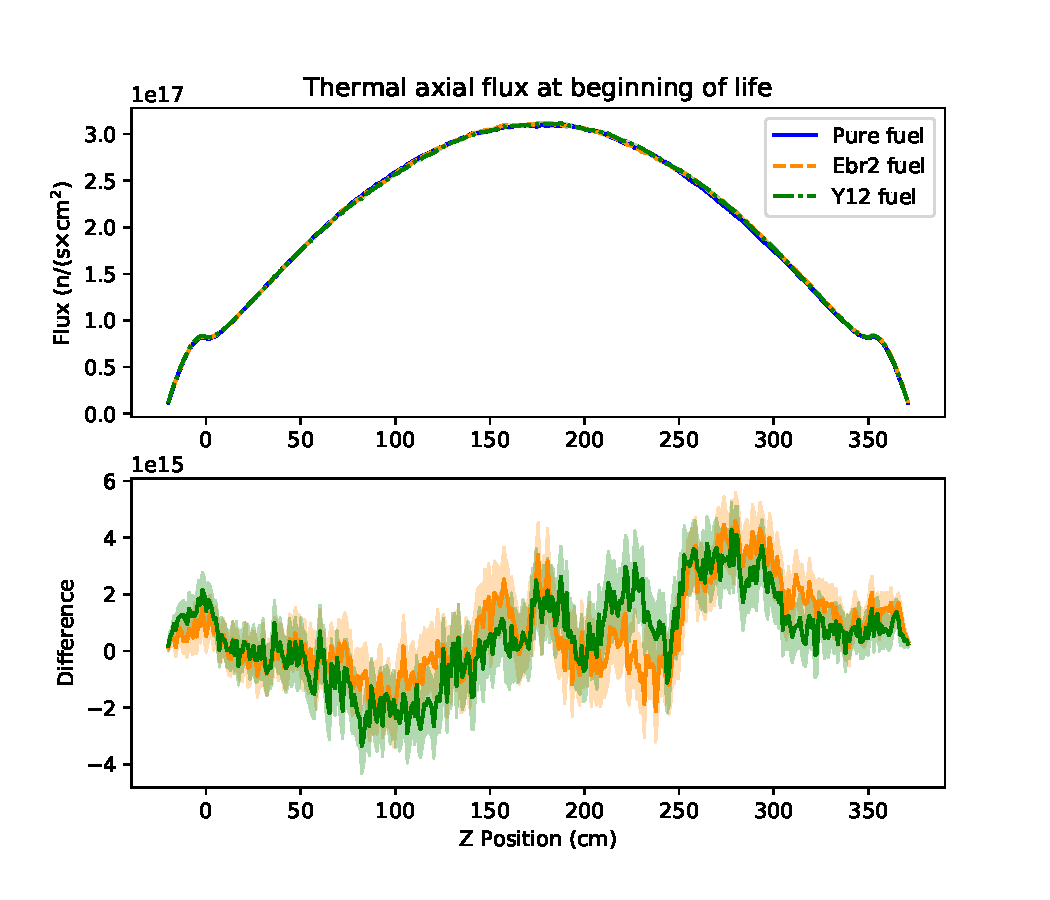
\includegraphics[width=\textwidth]{mmr_thermal_axial_bol.pdf}
            \caption{Thermal axial flux in the \gls{MMR}-like reactor. }
            \label{fig:mmr_thermal_axial_bol}
        \end{subfigure}
        \hfill
        \begin{subfigure}[b]{0.48\textwidth}
            \centering
            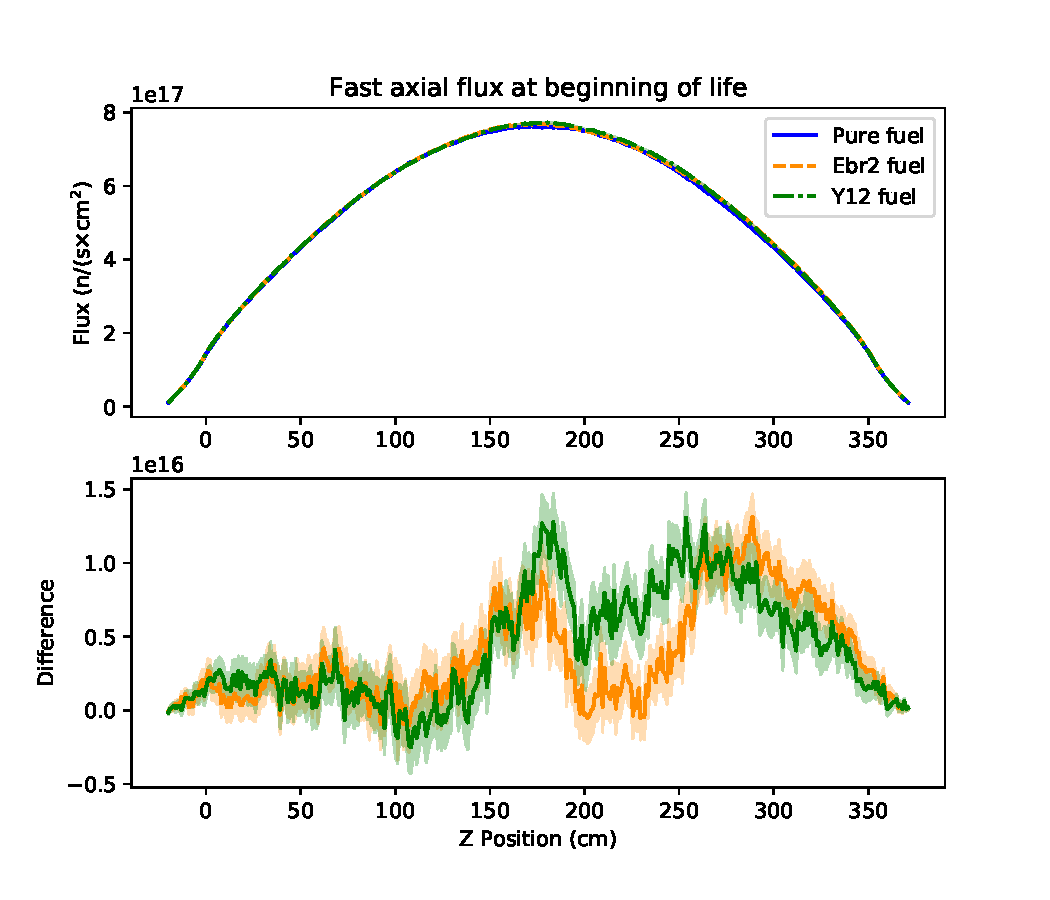
\includegraphics[width=\textwidth]{mmr_fast_axial_bol.pdf}
            \caption{Fast axial flux in the \gls{MMR}-like reactor.}
            \label{fig:mmr_fast_axial_bol}
        \end{subfigure}
        \hfill
        \caption{Radial and axial flux for each energy group when using 
        each fuel composition in the \gls{MMR}-like model at the beginning 
        of life. The thermal flux encompasses energies below 0.625 eV, and the 
        fast flux encompasses energies above 0.625 eV.}
        \label{fig:mmr_bol}
   \end{figure}

The axial fluxes at \gls{BOL} (Figures \ref{fig:mmr_thermal_axial_bol} and 
\ref{fig:mmr_fast_axial_bol}) show the effect of the graphite moderators at 
the top and bottom of the core. The thermal flux has a small peak in the 
moderator while the fast flux has a small exponential decrease in the 
moderator. The fluxes also show that using the impure fuels results in 
a slightly smaller flux at the bottom of the core and a slightly higher 
flux at the top of the core. The differences between the 
fluxes is 1-2 orders of magnitude smaller than the flux, but is 
still one order of magnitude larger than the error of the fluxes.

Figure \ref{fig:mmr_mc} shows the different fluxes in the \gls{MMR}-like 
reactor at \gls{MOL}. The trends at mid-cycle in the radial fluxes are 
similar to those observed at the \gls{BOL}: the radial fluxes have the 
greatest difference near the fuel pins in the core. In the axial fluxes 
however, there is a noticeable difference between the flux from the \gls{EBR} 
fuel and the other fuels. The \gls{EBR} results in a greater difference 
from the flux from the pure fuel than the Y-12 fuel, but the shape of 
the difference is similar to what was observed at \gls{BOL}; the flux from 
the \gls{EBR} fuel is less than the flux from the pure fuel in the bottom of 
the core and greater at the top of the core. For the thermal axial flux, 
the difference between the flux from the pure and Y-12 fuels decreases 
compared with the fluxes at \gls{BOL}, but the difference between the flux 
from pure and \gls{EBR} fuel increases compared with the flux at \gls{BOL}. 
A similar pattern occurs in the fast axial flux. This suggests that 
as the core burns, the impurities in the Y-12 fuel are burned off sooner 
than those present in the \gls{EBR} or that the impurities breed material 
similar to what is present in the pure fuel as it burns. 

\begin{figure}[h!]
        \centering
        \begin{subfigure}[b]{0.48\textwidth}
            \centering
            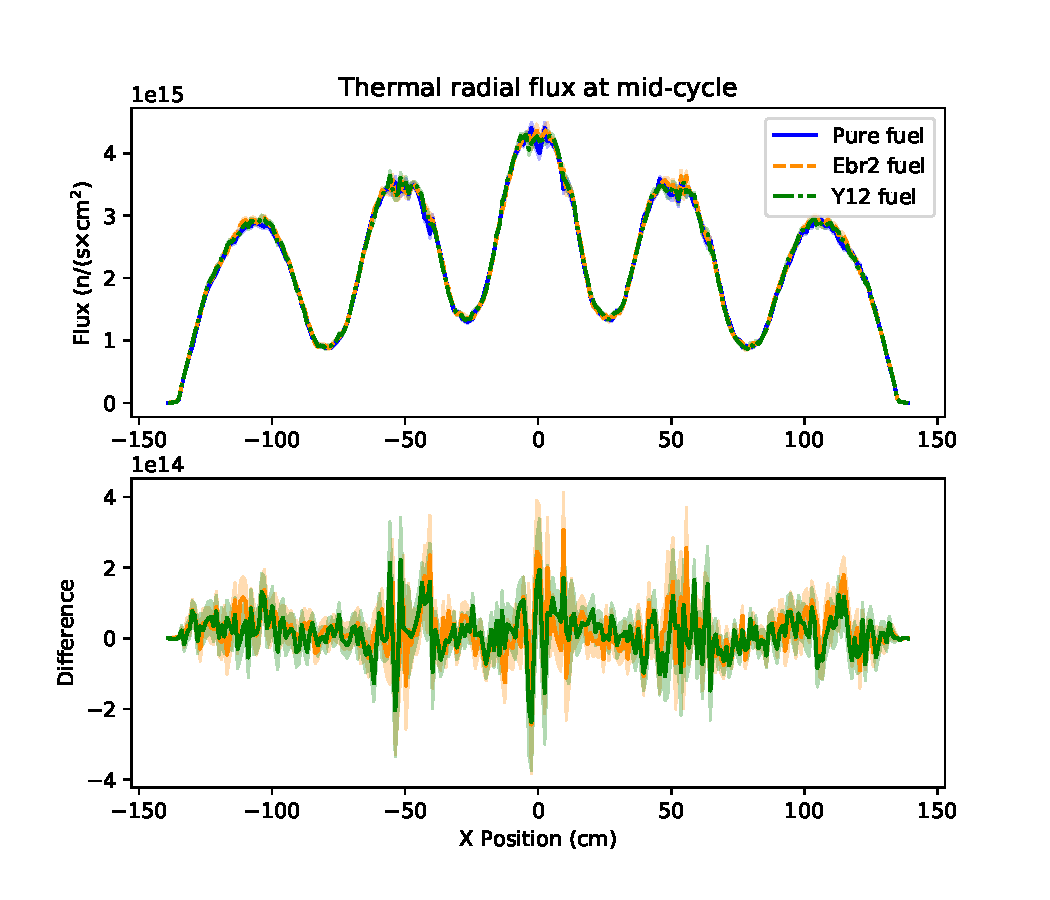
\includegraphics[width=\textwidth]{mmr_thermal_radial_mc.pdf}
            \caption{Thermal radial flux in the \gls{MMR}-like reactor.}
            \label{fig:mmr_thermal_radial_mc}
        \end{subfigure}
        \hfill
        \begin{subfigure}[b]{0.48\textwidth}
            \centering
            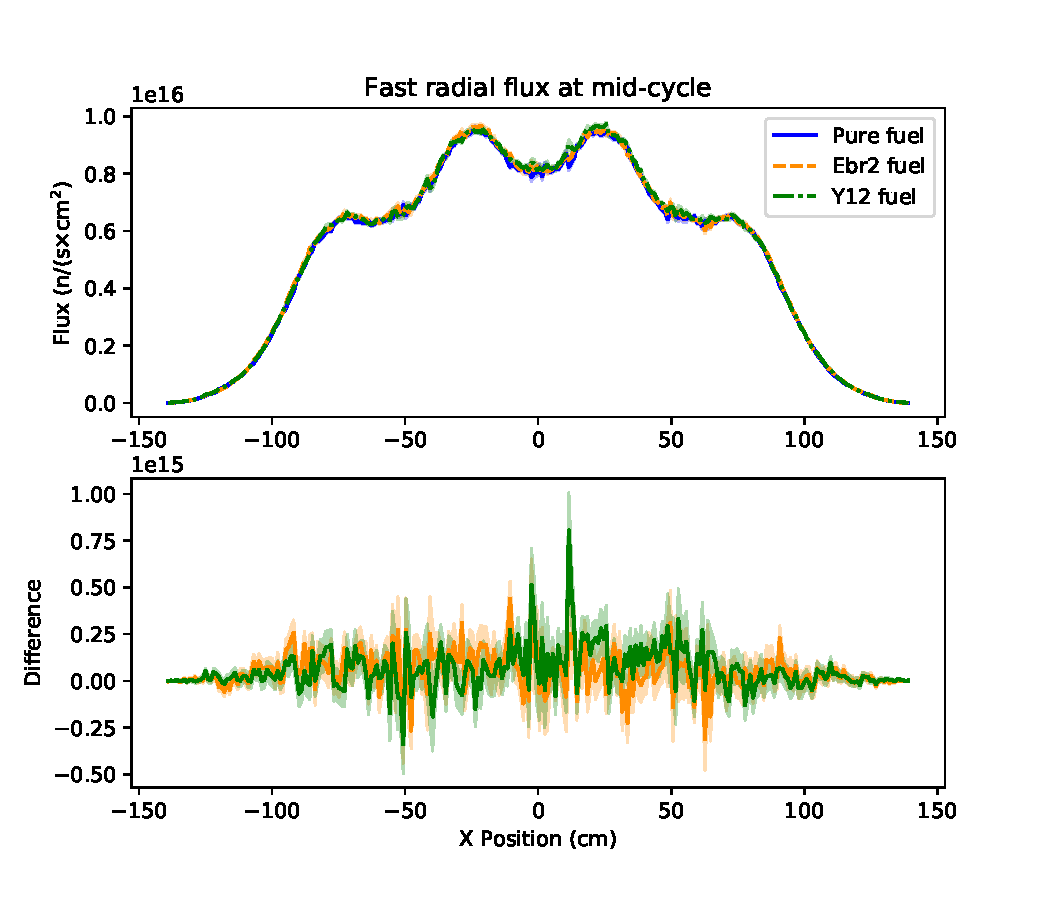
\includegraphics[width=\textwidth]{mmr_fast_radial_mc.pdf}
            \caption{Fast radial flux in the \gls{MMR}-like reactor.}
            \label{fig:mmr_fast_radial_mc}
        \end{subfigure}
        \hfill
            
        \begin{subfigure}[b]{0.48\textwidth}
            \centering
            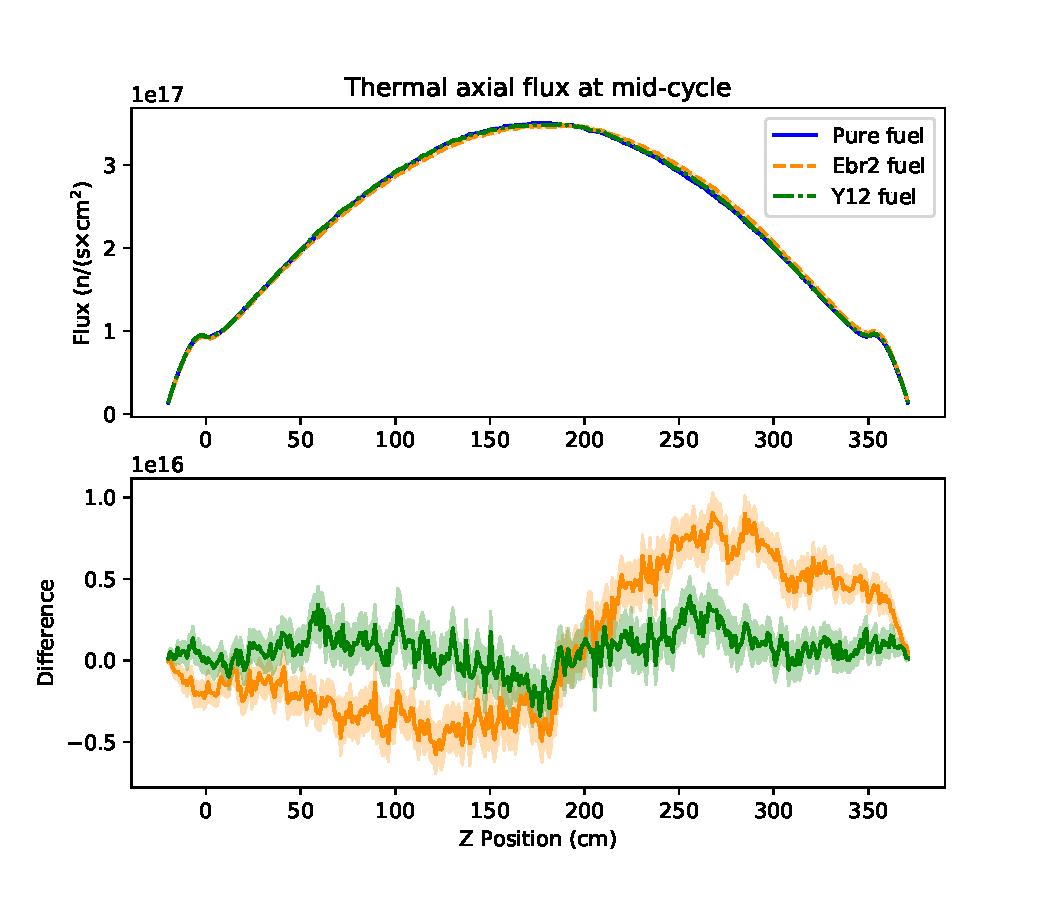
\includegraphics[width=\textwidth]{mmr_thermal_axial_mc.pdf}
            \caption{Thermal axial flux in the \gls{MMR}-like reactor. }
            \label{fig:mmr_thermal_axial_mc}
        \end{subfigure}
        \hfill
        \begin{subfigure}[b]{0.48\textwidth}
            \centering
            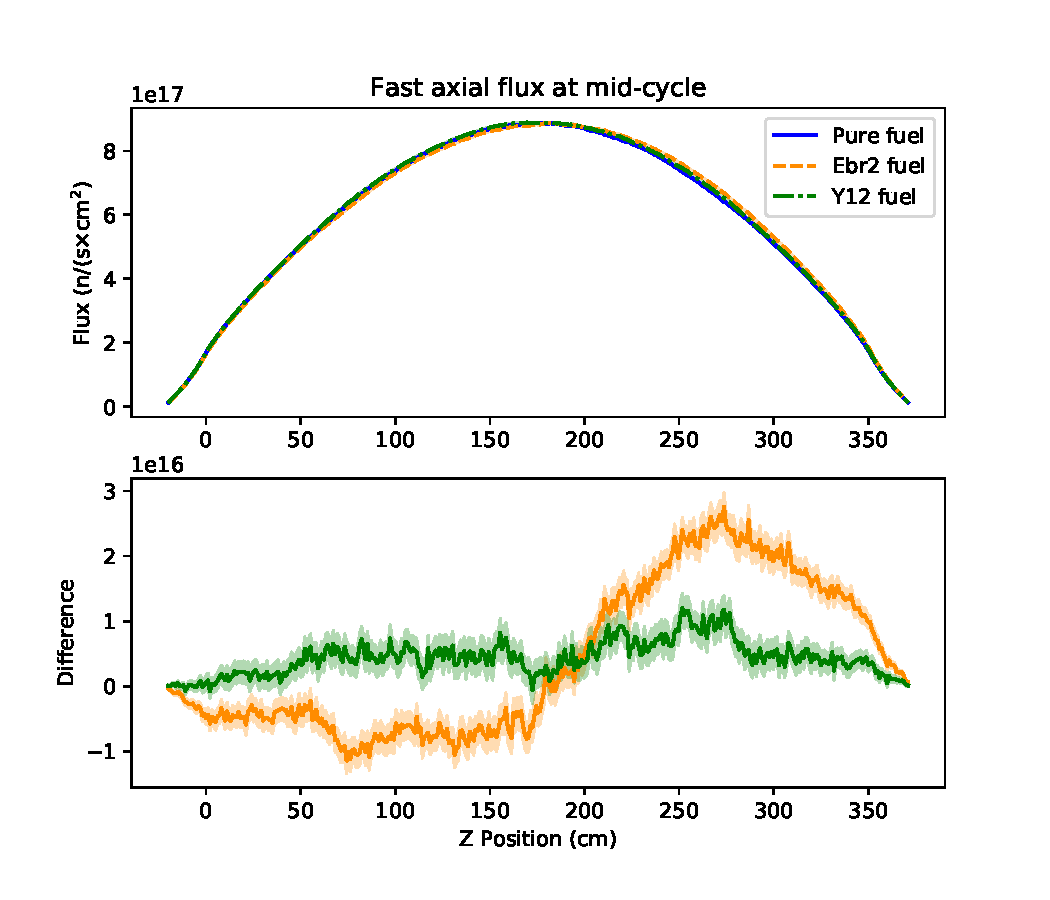
\includegraphics[width=\textwidth]{mmr_fast_axial_mc.pdf}
            \caption{Fast axial flux in the \gls{MMR}-like reactor.}
            \label{fig:mmr_fast_axial_mc}
        \end{subfigure}
        \hfill
        \caption{Radial and axial flux for each energy group when using 
        each fuel composition in the \gls{MMR}-like model at middle of 
        the operation cycle. The thermal flux encompasses energies below 
        0.625 eV, and the 
        fast flux encompasses energies above 0.625 eV.}
        \label{fig:mmr_mc}
   \end{figure}

Finally, Figure \ref{fig:mmr_eol} shows the different fluxes in the 
\gls{MMR}-like model at \gls{EOL}. The radial fluxes continue to show 
the same trend of the largest differences between the fluxes occurring near
the fuel pins. The axial fluxes (Figures \ref{fig:mmr_thermal_axial_eol} and 
\ref{fig:mmr_fast_axial_eol}) show a different trend. Both axial 
fluxes show that the impure fuels result in a larger flux at the 
bottom of the core and a smaller flux at the top of the core than the flux 
from the pure fuel, opposite
to what was observed in the \gls{BOL} and \gls{MOL} fluxes. The thermal 
and fast axial fluxes are higher at the \gls{EOL} than at the other 
two burnup steps. The difference between the flux from \gls{EBR} fuel 
and the pure fuel decreases from the difference at \gls{MOL}, but the 
difference between the fluxes from the pure and Y-12 fuel 
increases from the difference at \gls{MOL}. 
   
\begin{figure}[h!]
        \centering
        \begin{subfigure}[b]{0.48\textwidth}
            \centering
            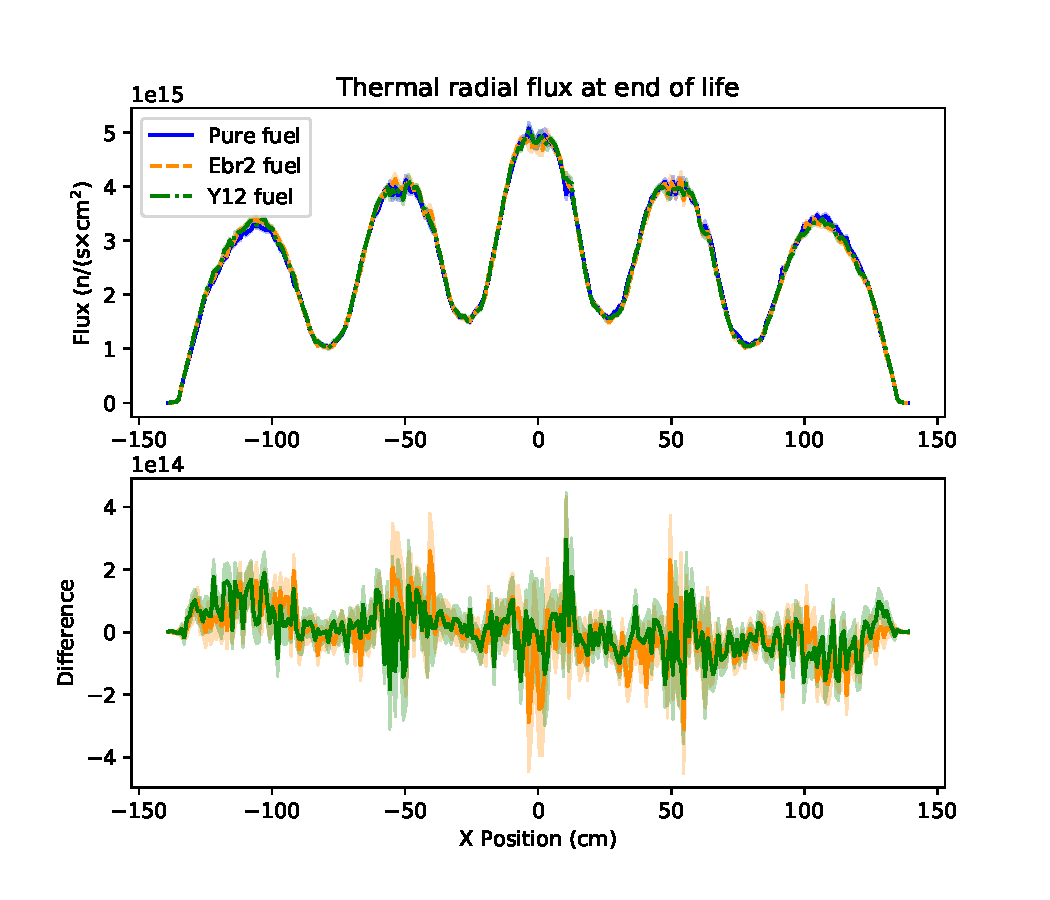
\includegraphics[width=\textwidth]{mmr_thermal_radial_eol.pdf}
            \caption{Thermal radial flux in the \gls{MMR}-like reactor.}
            \label{fig:mmr_thermal_radial_eol}
        \end{subfigure}
        \hfill
        \begin{subfigure}[b]{0.48\textwidth}
            \centering
            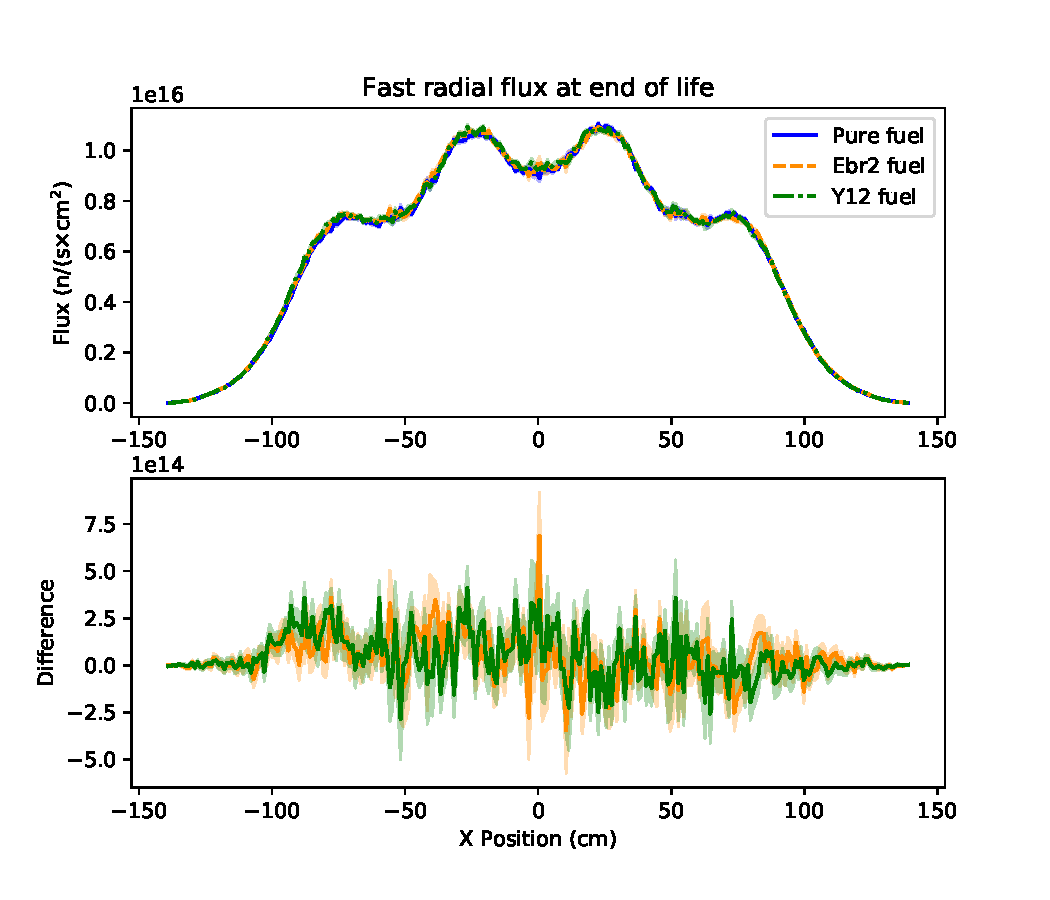
\includegraphics[width=\textwidth]{mmr_fast_radial_eol.pdf}
            \caption{Fast radial flux in the \gls{MMR}-like reactor.}
            \label{fig:mmr_fast_radial_eol}
        \end{subfigure}
        \hfill
            
        \begin{subfigure}[b]{0.48\textwidth}
            \centering
            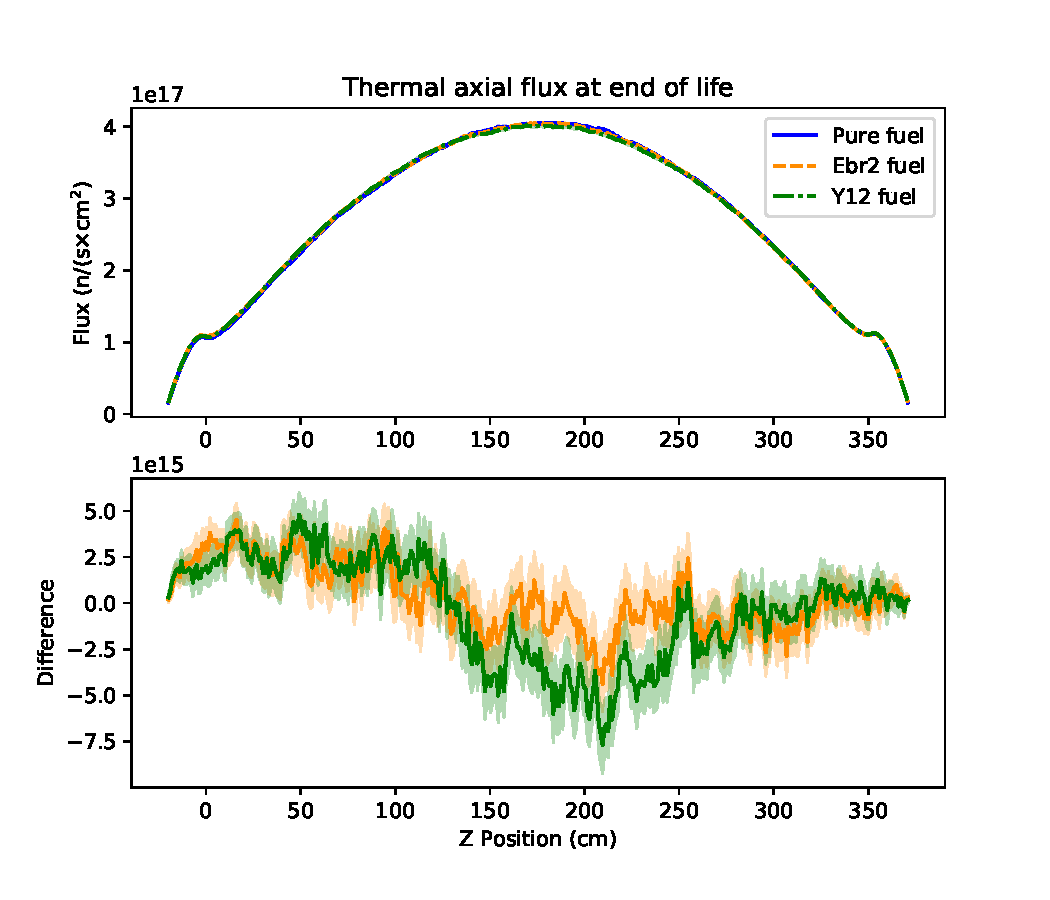
\includegraphics[width=\textwidth]{mmr_thermal_axial_eol.pdf}
            \caption{Thermal axial flux in the \gls{MMR}-like reactor. }
            \label{fig:mmr_thermal_axial_eol}
        \end{subfigure}
        \hfill
        \begin{subfigure}[b]{0.48\textwidth}
            \centering
            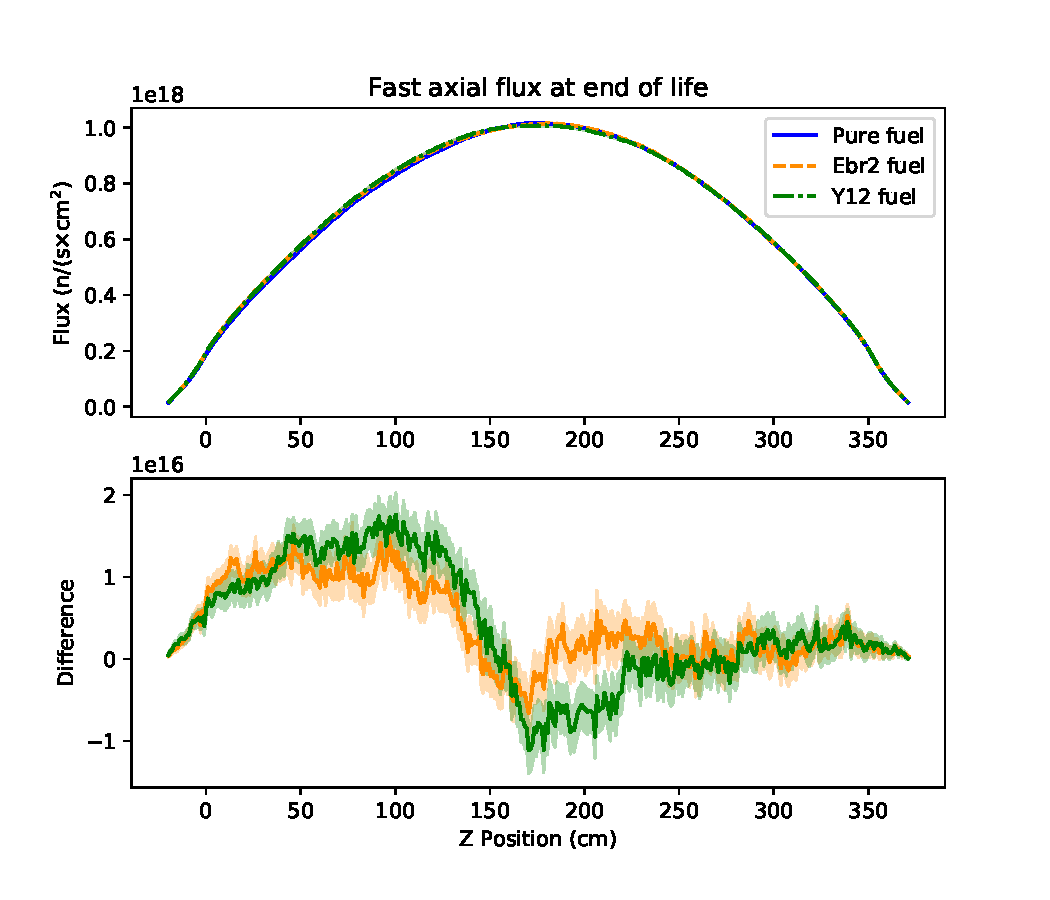
\includegraphics[width=\textwidth]{mmr_fast_axial_eol.pdf}
            \caption{Fast axial flux in the \gls{MMR}-like reactor.}
            \label{fig:mmr_fast_axial_eol}
        \end{subfigure}
        \hfill
        \caption{Radial and axial flux for each energy group when using 
        each fuel composition in the \gls{MMR}-like model at the end 
        of life. The thermal flux encompasses energies below 
        0.625 eV, and the 
        fast flux encompasses energies above 0.625 eV.}
        \label{fig:mmr_eol}
   \end{figure}


\subsubsection{Reactivity feedback coefficient comparison}
Finally, the reactivity feedback coefficients of different materials 
at each burnup step are reported in Table \ref{tab:coeff_mmr}. The 
fuel reactivity feedback coefficients become more negative with 
burnup, because the $^{235}$U in the core depleted with burnup, 
leaving a larger relative abundance of $^{238}$U and $^{239}$Pu in 
the core, which both have more resonances than $^{235}$U. The 
additional resonances of the $^{238}$U and $^{239}$Pu means that the 
Doppler broadening effect has a more pronounced impact on the reactivity 
of the core. At each of the burnup steps, the different fuel compositions 
result in different fuel reactivity coefficients, but each of the values 
are within error of each other. The values being within error suggests 
that the fuel composition does not have a significant effect on 
this parameter. 

\begin{table}[ht]
        \centering 
        \caption{Reactivity feedback coefficients (pcm/K) for different 
        materials at different burnup steps in the \gls{MMR}-like 
        reactor model.}
        \label{tab:coeff_mmr}
        \begin{tabular}{c c c c}
                \hline 
                & \multicolumn{3}{c}{Burnup step} \\
                Fuel & \gls{BOL} & \gls{MOL} & \gls{EOL} \\
                \hline 
                \multicolumn{4}{c}{Fuel reactivity feedabck}\\
                Pure & -3.314 $\pm$ 0.059 & -3.889 $\pm$ 0.088 & -4.536 $\pm$0.264\\
                \gls{EBR} & -3.073 $\pm$ 0.109 & -3.720 $\pm$ 0.147 & -4.699 $\pm$ 0.151\\
                Y-12 & -3.233 $\pm$ 0.107 & -3.704 $\pm$ 0.133 & -4.168 $\pm$ 0.100\\
                \hline 
                \multicolumn{4}{c}{Coolant reactivity feedabck}\\
                Pure & -0.211 $\pm$ 0.063 & 0.021 $\pm$ 0.169 & 0.052 $\pm$ 0.234\\
                \gls{EBR} & 0.007 $\pm$ 0.051 & -0.165 $\pm$ 0.183 & 0.005 $\pm$ 0.085\\
                Y-12 & -0.221 $\pm$ 0.068 & 0.197 $\pm$ 0.145 & -0.0146 $\pm$ 0.158\\
                \hline 
                \multicolumn{4}{c}{Moderator reactivity feedabck}\\
                Pure & -0.815 $\pm$ 0.062 & -1.298 $\pm$ 0.155 & -2.590 $\pm$ 0.323\\
                \gls{EBR} &-0.934 $\pm$ 0.171 & -1.723 $\pm$ 0.268 & -2.375 $\pm$ 0.313\\
                Y-12 & -0.950 $\pm$ 0.138 & -1.333 $\pm$ 0.206 & -2.432 $\pm$ 0.190\\
                \hline 
                \multicolumn{4}{c}{Total reactivity feedabck}\\
                Pure & -4.142 $\pm$ 0.297 & -5.015 $\pm$ 0.215 & -6.865 $\pm$ 0.300\\
                \gls{EBR} & -4.191 $\pm$ 0.097 & -5.284 $\pm$ 0.286 & -6.709 $\pm$ 0.329\\
                Y-12 & -4.037 $\pm$ 0.322 & -5.410 $\pm$ 0.268 & -6.689 $\pm$ 0.232\\
                \hline 
                
                
        \end{tabular}
\end{table}

The coolant reactivity feedback coefficients have the smallest absolute 
value of any of the coefficients considered in this work, which 
indicates that the helium coolant has the smallest effect on the reactivity 
of the core as the temperature changes. Additionally, the coolant 
reactivity feedback coefficient is not as dependent on the burnup of the 
fuel like the other coefficients, resulting from the density change 
being the primary temperature-dependent property of the helium coolant 
instead of widening of cross section resonances. 
At the \gls{BOL}, the \gls{EBR} fuel results in a statistically different 
coolant feedback coefficient, which shows that the fuel composition has some 
impact on this parameter. However, the coolant reactivity feedback 
coefficient is small compared to the other feedback coefficients so this 
change is unlikely to cause significant changes in the operation of the 
core as a whole. 

The moderator feedback coefficient is negative for each of the fuel 
compositions at each burnup step, indicating that this core is 
undermoderated. This feedback coefficient also becomes more 
negative with burnup, because the flux in the core increases with 
burnup. The increase in flux could be a result from the resonance 
broadening having more of an effect on the reactivity of the core, the 
density change of the graphite, or other effects. At the \gls{BOL} and 
\gls{MOL} steps the pure fuel has the least negative moderator 
feedback coefficient, but at \gls{EOL} the pure fuel has the most 
negative coefficient. However, at each of the burnup steps the moderator 
feedback coefficient from each of the fuels are within error of each 
other. This agreement within error suggests that the fuel composition 
does not have a significant effect on this reactor operation parameter. 

Finally, the total reactivity feedback coefficients are also all negative 
for each fuel composition at each burnup step, and they become more 
negative with burnup. Based on the values of the feedback 
coefficients for each individual material, the total feedback coefficient 
is mostly driven by the fuel feedback coefficient at each burnup step. 
The different fuel compositions result in total reactivity feedback 
coefficients that are within error of each other. Therefore, the fuel 
composition does not significantly affect this reactor parameter either. 

At each burnup step, the fuel and total reactivity feedback coefficients are 
negative for each fuel composition and the values from each fuel composition 
are within error of each other. These two results suggests that using any 
of these three fuel composition will not prevent this reactor design from 
operating in a safe state. 